\documentclass[1p]{elsarticle_modified}
%\bibliographystyle{elsarticle-num}

%\usepackage[colorlinks]{hyperref}
%\usepackage{abbrmath_seonhwa} %\Abb, \Ascr, \Acal ,\Abf, \Afrak
\usepackage{amsfonts}
\usepackage{amssymb}
\usepackage{amsmath}
\usepackage{amsthm}
\usepackage{scalefnt}
\usepackage{amsbsy}
\usepackage{kotex}
\usepackage{caption}
\usepackage{subfig}
\usepackage{color}
\usepackage{graphicx}
\usepackage{xcolor} %% white, black, red, green, blue, cyan, magenta, yellow
\usepackage{float}
\usepackage{setspace}
\usepackage{hyperref}

\usepackage{tikz}
\usetikzlibrary{arrows}

\usepackage{multirow}
\usepackage{array} % fixed length table
\usepackage{hhline}

%%%%%%%%%%%%%%%%%%%%%
\makeatletter
\renewcommand*\env@matrix[1][\arraystretch]{%
	\edef\arraystretch{#1}%
	\hskip -\arraycolsep
	\let\@ifnextchar\new@ifnextchar
	\array{*\c@MaxMatrixCols c}}
\makeatother %https://tex.stackexchange.com/questions/14071/how-can-i-increase-the-line-spacing-in-a-matrix
%%%%%%%%%%%%%%%

\usepackage[normalem]{ulem}

\newcommand{\msout}[1]{\ifmmode\text{\sout{\ensuremath{#1}}}\else\sout{#1}\fi}
%SOURCE: \msout is \stkout macro in https://tex.stackexchange.com/questions/20609/strikeout-in-math-mode

\newcommand{\cancel}[1]{
	\ifmmode
	{\color{red}\msout{#1}}
	\else
	{\color{red}\sout{#1}}
	\fi
}

\newcommand{\add}[1]{
	{\color{blue}\uwave{#1}}
}

\newcommand{\replace}[2]{
	\ifmmode
	{\color{red}\msout{#1}}{\color{blue}\uwave{#2}}
	\else
	{\color{red}\sout{#1}}{\color{blue}\uwave{#2}}
	\fi
}

\newcommand{\Sol}{\mathcal{S}} %segment
\newcommand{\D}{D} %diagram
\newcommand{\A}{\mathcal{A}} %arc


%%%%%%%%%%%%%%%%%%%%%%%%%%%%%5 test

\def\sl{\operatorname{\textup{SL}}(2,\Cbb)}
\def\psl{\operatorname{\textup{PSL}}(2,\Cbb)}
\def\quan{\mkern 1mu \triangleright \mkern 1mu}

\theoremstyle{definition}
\newtheorem{thm}{Theorem}[section]
\newtheorem{prop}[thm]{Proposition}
\newtheorem{lem}[thm]{Lemma}
\newtheorem{ques}[thm]{Question}
\newtheorem{cor}[thm]{Corollary}
\newtheorem{defn}[thm]{Definition}
\newtheorem{exam}[thm]{Example}
\newtheorem{rmk}[thm]{Remark}
\newtheorem{alg}[thm]{Algorithm}

\newcommand{\I}{\sqrt{-1}}
\begin{document}

%\begin{frontmatter}
%
%\title{Boundary parabolic representations of knots up to 8 crossings}
%
%%% Group authors per affiliation:
%\author{Yunhi Cho} 
%\address{Department of Mathematics, University of Seoul, Seoul, Korea}
%\ead{yhcho@uos.ac.kr}
%
%
%\author{Seonhwa Kim} %\fnref{s_kim}}
%\address{Center for Geometry and Physics, Institute for Basic Science, Pohang, 37673, Korea}
%\ead{ryeona17@ibs.re.kr}
%
%\author{Hyuk Kim}
%\address{Department of Mathematical Sciences, Seoul National University, Seoul 08826, Korea}
%\ead{hyukkim@snu.ac.kr}
%
%\author{Seokbeom Yoon}
%\address{Department of Mathematical Sciences, Seoul National University, Seoul, 08826,  Korea}
%\ead{sbyoon15@snu.ac.kr}
%
%\begin{abstract}
%We find all boundary parabolic representation of knots up to 8 crossings.
%
%\end{abstract}
%\begin{keyword}
%    \MSC[2010] 57M25 
%\end{keyword}
%
%\end{frontmatter}

%\linenumbers
%\tableofcontents
%
\newcommand\colored[1]{\textcolor{white}{\rule[-0.35ex]{0.8em}{1.4ex}}\kern-0.8em\color{red} #1}%
%\newcommand\colored[1]{\textcolor{white}{ #1}\kern-2.17ex	\textcolor{white}{ #1}\kern-1.81ex	\textcolor{white}{ #1}\kern-2.15ex\color{red}#1	}

{\Large $\underline{12a_{0754}~(K12a_{0754})}$}

\setlength{\tabcolsep}{10pt}
\renewcommand{\arraystretch}{1.6}
\vspace{1cm}\begin{tabular}{m{100pt}>{\centering\arraybackslash}m{274pt}}
\multirow{5}{120pt}{
	\centering
	\includegraphics[width=112pt]{../../../GIT/diagram.site/Diagrams/png/1555_12a_0754.png}\\
\ \ \ A knot diagram\footnotemark}&
\allowdisplaybreaks
\textbf{Linearized knot diagam} \\
\cline{2-2}
 &
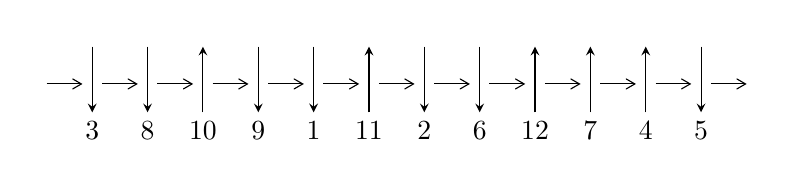
\begin{tikzpicture}[x=20pt, y=17pt]
	% nodes
	\node (C0) at (0, 0) {};
	\node (C1) at (1, 0) {};
	\node (C1U) at (1, +1) {};
	\node (C1D) at (1, -1) {3};

	\node (C2) at (2, 0) {};
	\node (C2U) at (2, +1) {};
	\node (C2D) at (2, -1) {8};

	\node (C3) at (3, 0) {};
	\node (C3U) at (3, +1) {};
	\node (C3D) at (3, -1) {10};

	\node (C4) at (4, 0) {};
	\node (C4U) at (4, +1) {};
	\node (C4D) at (4, -1) {9};

	\node (C5) at (5, 0) {};
	\node (C5U) at (5, +1) {};
	\node (C5D) at (5, -1) {1};

	\node (C6) at (6, 0) {};
	\node (C6U) at (6, +1) {};
	\node (C6D) at (6, -1) {11};

	\node (C7) at (7, 0) {};
	\node (C7U) at (7, +1) {};
	\node (C7D) at (7, -1) {2};

	\node (C8) at (8, 0) {};
	\node (C8U) at (8, +1) {};
	\node (C8D) at (8, -1) {6};

	\node (C9) at (9, 0) {};
	\node (C9U) at (9, +1) {};
	\node (C9D) at (9, -1) {12};

	\node (C10) at (10, 0) {};
	\node (C10U) at (10, +1) {};
	\node (C10D) at (10, -1) {7};

	\node (C11) at (11, 0) {};
	\node (C11U) at (11, +1) {};
	\node (C11D) at (11, -1) {4};

	\node (C12) at (12, 0) {};
	\node (C12U) at (12, +1) {};
	\node (C12D) at (12, -1) {5};
	\node (C13) at (13, 0) {};

	% arrows
	\draw[->,>={angle 60}]
	(C0) edge (C1) (C1) edge (C2) (C2) edge (C3) (C3) edge (C4) (C4) edge (C5) (C5) edge (C6) (C6) edge (C7) (C7) edge (C8) (C8) edge (C9) (C9) edge (C10) (C10) edge (C11) (C11) edge (C12) (C12) edge (C13) ;	\draw[->,>=stealth]
	(C1U) edge (C1D) (C2U) edge (C2D) (C3D) edge (C3U) (C4U) edge (C4D) (C5U) edge (C5D) (C6D) edge (C6U) (C7U) edge (C7D) (C8U) edge (C8D) (C9D) edge (C9U) (C10D) edge (C10U) (C11D) edge (C11U) (C12U) edge (C12D) ;
	\end{tikzpicture} \\
\hhline{~~} \\& 
\textbf{Solving Sequence} \\ \cline{2-2} 
 &
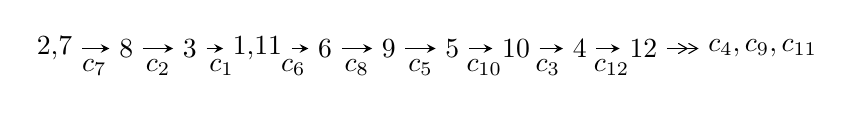
\begin{tikzpicture}[x=23pt, y=7pt]
	% node
	\node (A0) at (-1/8, 0) {2,7};
	\node (A1) at (1, 0) {8};
	\node (A2) at (2, 0) {3};
	\node (A3) at (49/16, 0) {1,11};
	\node (A4) at (33/8, 0) {6};
	\node (A5) at (41/8, 0) {9};
	\node (A6) at (49/8, 0) {5};
	\node (A7) at (57/8, 0) {10};
	\node (A8) at (65/8, 0) {4};
	\node (A9) at (73/8, 0) {12};
	\node (C1) at (1/2, -1) {$c_{7}$};
	\node (C2) at (3/2, -1) {$c_{2}$};
	\node (C3) at (5/2, -1) {$c_{1}$};
	\node (C4) at (29/8, -1) {$c_{6}$};
	\node (C5) at (37/8, -1) {$c_{8}$};
	\node (C6) at (45/8, -1) {$c_{5}$};
	\node (C7) at (53/8, -1) {$c_{10}$};
	\node (C8) at (61/8, -1) {$c_{3}$};
	\node (C9) at (69/8, -1) {$c_{12}$};
	\node (A10) at (11, 0) {$c_{4},c_{9},c_{11}$};

	% edge
	\draw[->,>=stealth]	
	(A0) edge (A1) (A1) edge (A2) (A2) edge (A3) (A3) edge (A4) (A4) edge (A5) (A5) edge (A6) (A6) edge (A7) (A7) edge (A8) (A8) edge (A9) ;
	\draw[->>,>={angle 60}]	
	(A9) edge (A10);
\end{tikzpicture} \\ 

\end{tabular} \\

\footnotetext{
The image of knot diagram is generated by the software ``\textbf{Draw programme}" developed by Andrew Bartholomew(\url{http://www.layer8.co.uk/maths/draw/index.htm\#Running-draw}), where we modified some parts for our purpose(\url{https://github.com/CATsTAILs/LinksPainter}).
}\phantom \\ \newline 
\centering \textbf{Ideals for irreducible components\footnotemark of $X_{\text{par}}$} 
 
\begin{align*}
I^u_{1}&=\langle 
-4.46501\times10^{559} u^{176}-3.76087\times10^{559} u^{175}+\cdots+3.16375\times10^{560} b-5.29003\times10^{561},\\
\phantom{I^u_{1}}&\phantom{= \langle  }-1.55061\times10^{560} u^{176}-1.24993\times10^{560} u^{175}+\cdots+6.89926\times10^{560} a-2.74571\times10^{562},\\
\phantom{I^u_{1}}&\phantom{= \langle  }u^{177}+u^{176}+\cdots-113 u+181\rangle \\
I^u_{2}&=\langle 
77050238748 u^{45}-49060443352 u^{44}+\cdots+31929802369 b-481900138262,\\
\phantom{I^u_{2}}&\phantom{= \langle  }-331992933622 u^{45}-546861658639 u^{44}+\cdots+31929802369 a+478475058213,\\
\phantom{I^u_{2}}&\phantom{= \langle  }u^{46}-14 u^{44}+\cdots+3 u+1\rangle \\
\\
\end{align*}
\raggedright * 2 irreducible components of $\dim_{\mathbb{C}}=0$, with total 223 representations.\\
\footnotetext{All coefficients of polynomials are rational numbers. But the coefficients are sometimes approximated in decimal forms when there is not enough margin.}
\newpage
\renewcommand{\arraystretch}{1}
\centering \section*{I. $I^u_{1}= \langle -4.47\times10^{559} u^{176}-3.76\times10^{559} u^{175}+\cdots+3.16\times10^{560} b-5.29\times10^{561},\;-1.55\times10^{560} u^{176}-1.25\times10^{560} u^{175}+\cdots+6.90\times10^{560} a-2.75\times10^{562},\;u^{177}+u^{176}+\cdots-113 u+181 \rangle$}
\flushleft \textbf{(i) Arc colorings}\\
\begin{tabular}{m{7pt} m{180pt} m{7pt} m{180pt} }
\flushright $a_{2}=$&$\begin{pmatrix}0\\u\end{pmatrix}$ \\
\flushright $a_{7}=$&$\begin{pmatrix}1\\0\end{pmatrix}$ \\
\flushright $a_{8}=$&$\begin{pmatrix}1\\u^2\end{pmatrix}$ \\
\flushright $a_{3}=$&$\begin{pmatrix}- u\\- u^3+u\end{pmatrix}$ \\
\flushright $a_{1}=$&$\begin{pmatrix}u^3\\u^5- u^3+u\end{pmatrix}$ \\
\flushright $a_{11}=$&$\begin{pmatrix}0.224751 u^{176}+0.181169 u^{175}+\cdots-91.7426 u+39.7972\\0.141130 u^{176}+0.118874 u^{175}+\cdots-50.5273 u+16.7208\end{pmatrix}$ \\
\flushright $a_{6}=$&$\begin{pmatrix}0.0966568 u^{176}+0.154708 u^{175}+\cdots+73.3219 u-43.4893\\0.0682880 u^{176}+0.0385578 u^{175}+\cdots+40.6569 u-20.0654\end{pmatrix}$ \\
\flushright $a_{9}=$&$\begin{pmatrix}0.110994 u^{176}+0.0695990 u^{175}+\cdots-132.292 u+49.7926\\0.0211045 u^{176}-0.0878728 u^{175}+\cdots-73.3585 u+41.7302\end{pmatrix}$ \\
\flushright $a_{5}=$&$\begin{pmatrix}-0.00914328 u^{176}+0.00801270 u^{175}+\cdots+86.7261 u-33.6343\\0.0205661 u^{176}-0.0320211 u^{175}+\cdots+30.3503 u-4.79365\end{pmatrix}$ \\
\flushright $a_{10}=$&$\begin{pmatrix}0.0836203 u^{176}+0.0622956 u^{175}+\cdots-41.2152 u+23.0764\\0.141130 u^{176}+0.118874 u^{175}+\cdots-50.5273 u+16.7208\end{pmatrix}$ \\
\flushright $a_{4}=$&$\begin{pmatrix}0.0277595 u^{176}+0.180289 u^{175}+\cdots-6.60090 u-14.9261\\-0.0125667 u^{176}+0.0103138 u^{175}+\cdots-29.9452 u+3.75498\end{pmatrix}$ \\
\flushright $a_{12}=$&$\begin{pmatrix}-0.0206965 u^{176}-0.105243 u^{175}+\cdots+42.4728 u+20.1661\\0.121159 u^{176}+0.164325 u^{175}+\cdots+14.5812 u-26.0587\end{pmatrix}$\\&\end{tabular}
\flushleft \textbf{(ii) Obstruction class $= -1$}\\~\\
\flushleft \textbf{(iii) Cusp Shapes $= 0.724599 u^{176}+1.40135 u^{175}+\cdots-17.4844 u-116.459$}\\~\\
\newpage\renewcommand{\arraystretch}{1}
\flushleft \textbf{(iv) u-Polynomials at the component}\newline \\
\begin{tabular}{m{50pt}|m{274pt}}
Crossings & \hspace{64pt}u-Polynomials at each crossing \\
\hline $$\begin{aligned}c_{1}\end{aligned}$$&$\begin{aligned}
&u^{177}+89 u^{176}+\cdots+1149811 u+32761
\end{aligned}$\\
\hline $$\begin{aligned}c_{2},c_{7}\end{aligned}$$&$\begin{aligned}
&u^{177}+u^{176}+\cdots-113 u+181
\end{aligned}$\\
\hline $$\begin{aligned}c_{3}\end{aligned}$$&$\begin{aligned}
&u^{177}+16 u^{175}+\cdots+2770141136 u+148430897
\end{aligned}$\\
\hline $$\begin{aligned}c_{4}\end{aligned}$$&$\begin{aligned}
&u^{177}+2 u^{176}+\cdots-118 u-47
\end{aligned}$\\
\hline $$\begin{aligned}c_{5},c_{12}\end{aligned}$$&$\begin{aligned}
&u^{177}-68 u^{175}+\cdots-8904 u+467
\end{aligned}$\\
\hline $$\begin{aligned}c_{6},c_{10}\end{aligned}$$&$\begin{aligned}
&u^{177}+51 u^{175}+\cdots+1008921 u+96053
\end{aligned}$\\
\hline $$\begin{aligned}c_{8}\end{aligned}$$&$\begin{aligned}
&u^{177}-10 u^{176}+\cdots+224156 u+83191
\end{aligned}$\\
\hline $$\begin{aligned}c_{9}\end{aligned}$$&$\begin{aligned}
&u^{177}+13 u^{176}+\cdots-3396057 u-216341
\end{aligned}$\\
\hline $$\begin{aligned}c_{11}\end{aligned}$$&$\begin{aligned}
&u^{177}-4 u^{176}+\cdots-500 u+41
\end{aligned}$\\
\hline
\end{tabular}\\~\\
\newpage\renewcommand{\arraystretch}{1}
\flushleft \textbf{(v) Riley Polynomials at the component}\newline \\
\begin{tabular}{m{50pt}|m{274pt}}
Crossings & \hspace{64pt}Riley Polynomials at each crossing \\
\hline $$\begin{aligned}c_{1}\end{aligned}$$&$\begin{aligned}
&y^{177}+15 y^{176}+\cdots+55508891787 y-1073283121
\end{aligned}$\\
\hline $$\begin{aligned}c_{2},c_{7}\end{aligned}$$&$\begin{aligned}
&y^{177}-89 y^{176}+\cdots+1149811 y-32761
\end{aligned}$\\
\hline $$\begin{aligned}c_{3}\end{aligned}$$&$\begin{aligned}
&y^{177}+32 y^{176}+\cdots-268829528448372104 y-22031731184224609
\end{aligned}$\\
\hline $$\begin{aligned}c_{4}\end{aligned}$$&$\begin{aligned}
&y^{177}-32 y^{176}+\cdots+102002 y-2209
\end{aligned}$\\
\hline $$\begin{aligned}c_{5},c_{12}\end{aligned}$$&$\begin{aligned}
&y^{177}-136 y^{176}+\cdots-143543164 y-218089
\end{aligned}$\\
\hline $$\begin{aligned}c_{6},c_{10}\end{aligned}$$&$\begin{aligned}
&y^{177}+102 y^{176}+\cdots-436351764825 y-9226178809
\end{aligned}$\\
\hline $$\begin{aligned}c_{8}\end{aligned}$$&$\begin{aligned}
&y^{177}-30 y^{176}+\cdots+663714149210 y-6920742481
\end{aligned}$\\
\hline $$\begin{aligned}c_{9}\end{aligned}$$&$\begin{aligned}
&y^{177}+43 y^{176}+\cdots-5046528559981 y-46803428281
\end{aligned}$\\
\hline $$\begin{aligned}c_{11}\end{aligned}$$&$\begin{aligned}
&y^{177}-14 y^{176}+\cdots+185384 y-1681
\end{aligned}$\\
\hline
\end{tabular}\\~\\
\newpage\flushleft \textbf{(vi) Complex Volumes and Cusp Shapes}
$$\begin{array}{c|c|c}  
\text{Solutions to }I^u_{1}& \I (\text{vol} + \sqrt{-1}CS) & \text{Cusp shape}\\
 \hline 
\begin{aligned}
u &= \phantom{-}0.974325 + 0.222085 I \\
a &= \phantom{-}0.81562 + 2.35721 I \\
b &= -0.09517 + 1.55029 I\end{aligned}
 & -6.50033 - 2.27440 I & \phantom{-0.000000 } 0 \\ \hline\begin{aligned}
u &= \phantom{-}0.974325 - 0.222085 I \\
a &= \phantom{-}0.81562 - 2.35721 I \\
b &= -0.09517 - 1.55029 I\end{aligned}
 & -6.50033 + 2.27440 I & \phantom{-0.000000 } 0 \\ \hline\begin{aligned}
u &= \phantom{-}0.995811 + 0.113591 I \\
a &= -0.03619 - 2.56105 I \\
b &= -0.210574 - 1.363500 I\end{aligned}
 & -6.60802 + 1.95285 I & \phantom{-0.000000 } 0 \\ \hline\begin{aligned}
u &= \phantom{-}0.995811 - 0.113591 I \\
a &= -0.03619 + 2.56105 I \\
b &= -0.210574 + 1.363500 I\end{aligned}
 & -6.60802 - 1.95285 I & \phantom{-0.000000 } 0 \\ \hline\begin{aligned}
u &= \phantom{-}0.891267 + 0.464106 I \\
a &= -1.80760 - 1.69279 I \\
b &= \phantom{-}0.148991 - 0.762299 I\end{aligned}
 & \phantom{-}0.290980 + 0.835797 I & \phantom{-0.000000 } 0 \\ \hline\begin{aligned}
u &= \phantom{-}0.891267 - 0.464106 I \\
a &= -1.80760 + 1.69279 I \\
b &= \phantom{-}0.148991 + 0.762299 I\end{aligned}
 & \phantom{-}0.290980 - 0.835797 I & \phantom{-0.000000 } 0 \\ \hline\begin{aligned}
u &= \phantom{-}0.932751 + 0.374408 I \\
a &= \phantom{-}0.347062 - 0.824795 I \\
b &= \phantom{-}1.238490 + 0.232968 I\end{aligned}
 & \phantom{-}0.20430 + 1.61888 I & \phantom{-0.000000 } 0 \\ \hline\begin{aligned}
u &= \phantom{-}0.932751 - 0.374408 I \\
a &= \phantom{-}0.347062 + 0.824795 I \\
b &= \phantom{-}1.238490 - 0.232968 I\end{aligned}
 & \phantom{-}0.20430 - 1.61888 I & \phantom{-0.000000 } 0 \\ \hline\begin{aligned}
u &= \phantom{-}0.249112 + 0.975833 I \\
a &= \phantom{-}0.059917 - 0.579235 I \\
b &= -0.401271 - 1.184370 I\end{aligned}
 & -5.10078 + 5.95524 I & \phantom{-0.000000 } 0 \\ \hline\begin{aligned}
u &= \phantom{-}0.249112 - 0.975833 I \\
a &= \phantom{-}0.059917 + 0.579235 I \\
b &= -0.401271 + 1.184370 I\end{aligned}
 & -5.10078 - 5.95524 I & \phantom{-0.000000 } 0\\
 \hline 
 \end{array}$$\newpage$$\begin{array}{c|c|c}  
\text{Solutions to }I^u_{1}& \I (\text{vol} + \sqrt{-1}CS) & \text{Cusp shape}\\
 \hline 
\begin{aligned}
u &= \phantom{-}0.659460 + 0.739964 I \\
a &= \phantom{-}0.265306 - 0.602206 I \\
b &= -0.602881 - 0.581728 I\end{aligned}
 & \phantom{-}0.50499 - 5.98199 I & \phantom{-0.000000 } 0 \\ \hline\begin{aligned}
u &= \phantom{-}0.659460 - 0.739964 I \\
a &= \phantom{-}0.265306 + 0.602206 I \\
b &= -0.602881 + 0.581728 I\end{aligned}
 & \phantom{-}0.50499 + 5.98199 I & \phantom{-0.000000 } 0 \\ \hline\begin{aligned}
u &= -0.960156 + 0.320973 I \\
a &= -2.51324 + 3.47680 I \\
b &= \phantom{-}0.036699 + 0.860470 I\end{aligned}
 & -4.97745 - 3.70596 I & \phantom{-0.000000 } 0 \\ \hline\begin{aligned}
u &= -0.960156 - 0.320973 I \\
a &= -2.51324 - 3.47680 I \\
b &= \phantom{-}0.036699 - 0.860470 I\end{aligned}
 & -4.97745 + 3.70596 I & \phantom{-0.000000 } 0 \\ \hline\begin{aligned}
u &= -0.327466 + 0.959605 I \\
a &= \phantom{-}0.373522 + 0.507460 I \\
b &= -0.623318 + 1.250290 I\end{aligned}
 & -3.9652 - 14.7921 I & \phantom{-0.000000 } 0 \\ \hline\begin{aligned}
u &= -0.327466 - 0.959605 I \\
a &= \phantom{-}0.373522 - 0.507460 I \\
b &= -0.623318 - 1.250290 I\end{aligned}
 & -3.9652 + 14.7921 I & \phantom{-0.000000 } 0 \\ \hline\begin{aligned}
u &= \phantom{-}0.873905 + 0.453283 I \\
a &= \phantom{-}0.18625 + 1.54037 I \\
b &= -1.080860 + 0.499009 I\end{aligned}
 & \phantom{-}0.24529 - 4.90883 I & \phantom{-0.000000 } 0 \\ \hline\begin{aligned}
u &= \phantom{-}0.873905 - 0.453283 I \\
a &= \phantom{-}0.18625 - 1.54037 I \\
b &= -1.080860 - 0.499009 I\end{aligned}
 & \phantom{-}0.24529 + 4.90883 I & \phantom{-0.000000 } 0 \\ \hline\begin{aligned}
u &= \phantom{-}0.407136 + 0.876029 I \\
a &= \phantom{-}0.228493 - 0.230111 I \\
b &= -0.625577 - 1.213760 I\end{aligned}
 & \phantom{-}0.65768 + 8.86127 I & \phantom{-0.000000 } 0 \\ \hline\begin{aligned}
u &= \phantom{-}0.407136 - 0.876029 I \\
a &= \phantom{-}0.228493 + 0.230111 I \\
b &= -0.625577 + 1.213760 I\end{aligned}
 & \phantom{-}0.65768 - 8.86127 I & \phantom{-0.000000 } 0\\
 \hline 
 \end{array}$$\newpage$$\begin{array}{c|c|c}  
\text{Solutions to }I^u_{1}& \I (\text{vol} + \sqrt{-1}CS) & \text{Cusp shape}\\
 \hline 
\begin{aligned}
u &= -0.929681 + 0.252073 I \\
a &= \phantom{-}1.98508 - 1.54026 I \\
b &= -0.101282 + 0.438544 I\end{aligned}
 & -4.69188 + 6.03218 I & \phantom{-0.000000 } 0 \\ \hline\begin{aligned}
u &= -0.929681 - 0.252073 I \\
a &= \phantom{-}1.98508 + 1.54026 I \\
b &= -0.101282 - 0.438544 I\end{aligned}
 & -4.69188 - 6.03218 I & \phantom{-0.000000 } 0 \\ \hline\begin{aligned}
u &= -0.891310 + 0.531806 I \\
a &= -0.659025 + 0.106796 I \\
b &= -0.613693 + 0.630340 I\end{aligned}
 & -0.962538 + 0.626000 I & \phantom{-0.000000 } 0 \\ \hline\begin{aligned}
u &= -0.891310 - 0.531806 I \\
a &= -0.659025 - 0.106796 I \\
b &= -0.613693 - 0.630340 I\end{aligned}
 & -0.962538 - 0.626000 I & \phantom{-0.000000 } 0 \\ \hline\begin{aligned}
u &= -0.484590 + 0.828041 I \\
a &= -0.455710 - 0.186890 I \\
b &= \phantom{-}0.390296 - 1.060170 I\end{aligned}
 & -1.27015 - 3.46858 I & \phantom{-0.000000 } 0 \\ \hline\begin{aligned}
u &= -0.484590 - 0.828041 I \\
a &= -0.455710 + 0.186890 I \\
b &= \phantom{-}0.390296 + 1.060170 I\end{aligned}
 & -1.27015 + 3.46858 I & \phantom{-0.000000 } 0 \\ \hline\begin{aligned}
u &= \phantom{-}0.981309 + 0.356252 I \\
a &= -0.0327071 - 0.1150610 I \\
b &= \phantom{-}0.825548 + 0.833562 I\end{aligned}
 & -4.80627 + 0.53223 I & \phantom{-0.000000 } 0 \\ \hline\begin{aligned}
u &= \phantom{-}0.981309 - 0.356252 I \\
a &= -0.0327071 + 0.1150610 I \\
b &= \phantom{-}0.825548 - 0.833562 I\end{aligned}
 & -4.80627 - 0.53223 I & \phantom{-0.000000 } 0 \\ \hline\begin{aligned}
u &= \phantom{-}0.801643 + 0.676667 I \\
a &= -0.535505 - 0.017695 I \\
b &= \phantom{-}0.469122 - 0.536520 I\end{aligned}
 & \phantom{-}3.06544 - 2.33212 I & \phantom{-0.000000 } 0 \\ \hline\begin{aligned}
u &= \phantom{-}0.801643 - 0.676667 I \\
a &= -0.535505 + 0.017695 I \\
b &= \phantom{-}0.469122 + 0.536520 I\end{aligned}
 & \phantom{-}3.06544 + 2.33212 I & \phantom{-0.000000 } 0\\
 \hline 
 \end{array}$$\newpage$$\begin{array}{c|c|c}  
\text{Solutions to }I^u_{1}& \I (\text{vol} + \sqrt{-1}CS) & \text{Cusp shape}\\
 \hline 
\begin{aligned}
u &= \phantom{-}0.997233 + 0.341494 I \\
a &= \phantom{-}1.00789 + 1.50673 I \\
b &= \phantom{-}0.56095 + 1.59851 I\end{aligned}
 & -7.10045 + 0.18077 I & \phantom{-0.000000 } 0 \\ \hline\begin{aligned}
u &= \phantom{-}0.997233 - 0.341494 I \\
a &= \phantom{-}1.00789 - 1.50673 I \\
b &= \phantom{-}0.56095 - 1.59851 I\end{aligned}
 & -7.10045 - 0.18077 I & \phantom{-0.000000 } 0 \\ \hline\begin{aligned}
u &= -0.425461 + 0.839516 I \\
a &= -0.655201 + 0.424317 I \\
b &= \phantom{-}0.541164 + 0.346849 I\end{aligned}
 & -1.55079 - 0.51771 I & \phantom{-0.000000 } 0 \\ \hline\begin{aligned}
u &= -0.425461 - 0.839516 I \\
a &= -0.655201 - 0.424317 I \\
b &= \phantom{-}0.541164 - 0.346849 I\end{aligned}
 & -1.55079 + 0.51771 I & \phantom{-0.000000 } 0 \\ \hline\begin{aligned}
u &= -0.672996 + 0.819837 I \\
a &= -0.809570 - 0.195709 I \\
b &= \phantom{-}0.293941 + 0.657252 I\end{aligned}
 & -0.20302 - 1.64601 I & \phantom{-0.000000 } 0 \\ \hline\begin{aligned}
u &= -0.672996 - 0.819837 I \\
a &= -0.809570 + 0.195709 I \\
b &= \phantom{-}0.293941 - 0.657252 I\end{aligned}
 & -0.20302 + 1.64601 I & \phantom{-0.000000 } 0 \\ \hline\begin{aligned}
u &= -0.936300\phantom{ +0.000000I} \\
a &= -1.21722\phantom{ +0.000000I} \\
b &= -0.597295\phantom{ +0.000000I}\end{aligned}
 & -2.21006\phantom{ +0.000000I} & \phantom{-0.000000 } 0 \\ \hline\begin{aligned}
u &= \phantom{-}0.546028 + 0.739177 I \\
a &= -0.91845 + 1.25629 I \\
b &= \phantom{-}0.353663 + 0.981728 I\end{aligned}
 & -1.28885 + 4.62079 I & \phantom{-0.000000 } 0 \\ \hline\begin{aligned}
u &= \phantom{-}0.546028 - 0.739177 I \\
a &= -0.91845 - 1.25629 I \\
b &= \phantom{-}0.353663 - 0.981728 I\end{aligned}
 & -1.28885 - 4.62079 I & \phantom{-0.000000 } 0 \\ \hline\begin{aligned}
u &= -0.652726 + 0.646500 I \\
a &= -0.619657 + 0.655257 I \\
b &= \phantom{-}0.623344 + 0.968272 I\end{aligned}
 & -0.26043 + 4.06910 I & \phantom{-0.000000 } 0\\
 \hline 
 \end{array}$$\newpage$$\begin{array}{c|c|c}  
\text{Solutions to }I^u_{1}& \I (\text{vol} + \sqrt{-1}CS) & \text{Cusp shape}\\
 \hline 
\begin{aligned}
u &= -0.652726 - 0.646500 I \\
a &= -0.619657 - 0.655257 I \\
b &= \phantom{-}0.623344 - 0.968272 I\end{aligned}
 & -0.26043 - 4.06910 I & \phantom{-0.000000 } 0 \\ \hline\begin{aligned}
u &= \phantom{-}0.865311 + 0.268129 I \\
a &= \phantom{-}1.34391 + 3.02315 I \\
b &= -0.518492 + 1.045400 I\end{aligned}
 & -4.20869 - 3.12674 I & \phantom{-0.000000 } 0 \\ \hline\begin{aligned}
u &= \phantom{-}0.865311 - 0.268129 I \\
a &= \phantom{-}1.34391 - 3.02315 I \\
b &= -0.518492 - 1.045400 I\end{aligned}
 & -4.20869 + 3.12674 I & \phantom{-0.000000 } 0 \\ \hline\begin{aligned}
u &= \phantom{-}0.019928 + 0.897306 I \\
a &= -1.023540 - 0.325536 I \\
b &= \phantom{-}0.438641 - 0.962197 I\end{aligned}
 & -4.15749 - 1.66209 I & \phantom{-0.000000 } 0 \\ \hline\begin{aligned}
u &= \phantom{-}0.019928 - 0.897306 I \\
a &= -1.023540 + 0.325536 I \\
b &= \phantom{-}0.438641 + 0.962197 I\end{aligned}
 & -4.15749 + 1.66209 I & \phantom{-0.000000 } 0 \\ \hline\begin{aligned}
u &= \phantom{-}0.984173 + 0.497443 I \\
a &= \phantom{-}0.525993 + 0.587716 I \\
b &= -0.548453 - 0.164878 I\end{aligned}
 & -0.21065 - 4.60175 I & \phantom{-0.000000 } 0 \\ \hline\begin{aligned}
u &= \phantom{-}0.984173 - 0.497443 I \\
a &= \phantom{-}0.525993 - 0.587716 I \\
b &= -0.548453 + 0.164878 I\end{aligned}
 & -0.21065 + 4.60175 I & \phantom{-0.000000 } 0 \\ \hline\begin{aligned}
u &= \phantom{-}0.870051 + 0.679152 I \\
a &= -0.313124 + 0.500964 I \\
b &= -0.323064 - 0.402527 I\end{aligned}
 & \phantom{-}2.87655 - 2.88564 I & \phantom{-0.000000 } 0 \\ \hline\begin{aligned}
u &= \phantom{-}0.870051 - 0.679152 I \\
a &= -0.313124 - 0.500964 I \\
b &= -0.323064 + 0.402527 I\end{aligned}
 & \phantom{-}2.87655 + 2.88564 I & \phantom{-0.000000 } 0 \\ \hline\begin{aligned}
u &= -1.023420 + 0.414546 I \\
a &= -0.59669 + 2.65233 I \\
b &= -0.25466 + 1.43283 I\end{aligned}
 & -8.30031 - 2.14999 I & \phantom{-0.000000 } 0\\
 \hline 
 \end{array}$$\newpage$$\begin{array}{c|c|c}  
\text{Solutions to }I^u_{1}& \I (\text{vol} + \sqrt{-1}CS) & \text{Cusp shape}\\
 \hline 
\begin{aligned}
u &= -1.023420 - 0.414546 I \\
a &= -0.59669 - 2.65233 I \\
b &= -0.25466 - 1.43283 I\end{aligned}
 & -8.30031 + 2.14999 I & \phantom{-0.000000 } 0 \\ \hline\begin{aligned}
u &= -1.003530 + 0.468682 I \\
a &= -1.007460 - 0.720630 I \\
b &= -1.249210 + 0.598406 I\end{aligned}
 & \phantom{-}0.280054 + 0.456269 I & \phantom{-0.000000 } 0 \\ \hline\begin{aligned}
u &= -1.003530 - 0.468682 I \\
a &= -1.007460 + 0.720630 I \\
b &= -1.249210 - 0.598406 I\end{aligned}
 & \phantom{-}0.280054 - 0.456269 I & \phantom{-0.000000 } 0 \\ \hline\begin{aligned}
u &= -0.982907 + 0.512624 I \\
a &= \phantom{-}1.30656 - 2.51647 I \\
b &= -0.358370 - 1.078470 I\end{aligned}
 & \phantom{-}0.86960 + 5.99499 I & \phantom{-0.000000 } 0 \\ \hline\begin{aligned}
u &= -0.982907 - 0.512624 I \\
a &= \phantom{-}1.30656 + 2.51647 I \\
b &= -0.358370 + 1.078470 I\end{aligned}
 & \phantom{-}0.86960 - 5.99499 I & \phantom{-0.000000 } 0 \\ \hline\begin{aligned}
u &= \phantom{-}0.664022 + 0.902110 I \\
a &= \phantom{-}0.268917 + 0.282201 I \\
b &= -0.314378 + 0.879919 I\end{aligned}
 & \phantom{-}2.10337 - 4.61954 I & \phantom{-0.000000 } 0 \\ \hline\begin{aligned}
u &= \phantom{-}0.664022 - 0.902110 I \\
a &= \phantom{-}0.268917 - 0.282201 I \\
b &= -0.314378 - 0.879919 I\end{aligned}
 & \phantom{-}2.10337 + 4.61954 I & \phantom{-0.000000 } 0 \\ \hline\begin{aligned}
u &= \phantom{-}0.352863 + 1.065400 I \\
a &= -0.443332 + 0.605358 I \\
b &= \phantom{-}0.486671 + 1.071910 I\end{aligned}
 & -3.61595 + 4.69476 I & \phantom{-0.000000 } 0 \\ \hline\begin{aligned}
u &= \phantom{-}0.352863 - 1.065400 I \\
a &= -0.443332 - 0.605358 I \\
b &= \phantom{-}0.486671 - 1.071910 I\end{aligned}
 & -3.61595 - 4.69476 I & \phantom{-0.000000 } 0 \\ \hline\begin{aligned}
u &= \phantom{-}0.367583 + 0.796928 I \\
a &= \phantom{-}0.589023 + 0.487069 I \\
b &= -1.048850 + 0.291504 I\end{aligned}
 & -0.95048 + 8.79821 I & \phantom{-0.000000 } 0\\
 \hline 
 \end{array}$$\newpage$$\begin{array}{c|c|c}  
\text{Solutions to }I^u_{1}& \I (\text{vol} + \sqrt{-1}CS) & \text{Cusp shape}\\
 \hline 
\begin{aligned}
u &= \phantom{-}0.367583 - 0.796928 I \\
a &= \phantom{-}0.589023 - 0.487069 I \\
b &= -1.048850 - 0.291504 I\end{aligned}
 & -0.95048 - 8.79821 I & \phantom{-0.000000 } 0 \\ \hline\begin{aligned}
u &= \phantom{-}1.123410 + 0.148227 I \\
a &= \phantom{-}0.147814 + 0.129479 I \\
b &= -0.463378 - 0.322398 I\end{aligned}
 & -6.76781 - 1.75341 I & \phantom{-0.000000 } 0 \\ \hline\begin{aligned}
u &= \phantom{-}1.123410 - 0.148227 I \\
a &= \phantom{-}0.147814 - 0.129479 I \\
b &= -0.463378 + 0.322398 I\end{aligned}
 & -6.76781 + 1.75341 I & \phantom{-0.000000 } 0 \\ \hline\begin{aligned}
u &= \phantom{-}0.861289 + 0.741903 I \\
a &= -0.87342 - 1.18739 I \\
b &= \phantom{-}0.441231 - 0.715211 I\end{aligned}
 & -0.091216 + 0.552522 I & \phantom{-0.000000 } 0 \\ \hline\begin{aligned}
u &= \phantom{-}0.861289 - 0.741903 I \\
a &= -0.87342 + 1.18739 I \\
b &= \phantom{-}0.441231 + 0.715211 I\end{aligned}
 & -0.091216 - 0.552522 I & \phantom{-0.000000 } 0 \\ \hline\begin{aligned}
u &= \phantom{-}1.086500 + 0.349977 I \\
a &= \phantom{-}0.21485 - 2.17760 I \\
b &= \phantom{-}0.020473 - 1.231930 I\end{aligned}
 & -8.19104 - 3.38162 I & \phantom{-0.000000 } 0 \\ \hline\begin{aligned}
u &= \phantom{-}1.086500 - 0.349977 I \\
a &= \phantom{-}0.21485 + 2.17760 I \\
b &= \phantom{-}0.020473 + 1.231930 I\end{aligned}
 & -8.19104 + 3.38162 I & \phantom{-0.000000 } 0 \\ \hline\begin{aligned}
u &= \phantom{-}1.027750 + 0.501132 I \\
a &= \phantom{-}2.55206 + 1.43844 I \\
b &= -0.338256 + 1.215810 I\end{aligned}
 & -7.70017 - 8.42877 I & \phantom{-0.000000 } 0 \\ \hline\begin{aligned}
u &= \phantom{-}1.027750 - 0.501132 I \\
a &= \phantom{-}2.55206 - 1.43844 I \\
b &= -0.338256 - 1.215810 I\end{aligned}
 & -7.70017 + 8.42877 I & \phantom{-0.000000 } 0 \\ \hline\begin{aligned}
u &= \phantom{-}1.012670 + 0.531949 I \\
a &= -0.213014 + 1.212140 I \\
b &= -1.113660 + 0.102945 I\end{aligned}
 & \phantom{-}0.56443 - 5.15617 I & \phantom{-0.000000 } 0\\
 \hline 
 \end{array}$$\newpage$$\begin{array}{c|c|c}  
\text{Solutions to }I^u_{1}& \I (\text{vol} + \sqrt{-1}CS) & \text{Cusp shape}\\
 \hline 
\begin{aligned}
u &= \phantom{-}1.012670 - 0.531949 I \\
a &= -0.213014 - 1.212140 I \\
b &= -1.113660 - 0.102945 I\end{aligned}
 & \phantom{-}0.56443 + 5.15617 I & \phantom{-0.000000 } 0 \\ \hline\begin{aligned}
u &= -1.135000 + 0.178422 I \\
a &= \phantom{-}0.406463 + 0.890434 I \\
b &= \phantom{-}0.901111 - 0.067709 I\end{aligned}
 & -5.88446 - 6.20711 I & \phantom{-0.000000 } 0 \\ \hline\begin{aligned}
u &= -1.135000 - 0.178422 I \\
a &= \phantom{-}0.406463 - 0.890434 I \\
b &= \phantom{-}0.901111 + 0.067709 I\end{aligned}
 & -5.88446 + 6.20711 I & \phantom{-0.000000 } 0 \\ \hline\begin{aligned}
u &= -1.115390 + 0.308103 I \\
a &= -0.91644 + 1.59936 I \\
b &= -0.400309 + 1.255670 I\end{aligned}
 & -3.51682 - 0.04625 I & \phantom{-0.000000 } 0 \\ \hline\begin{aligned}
u &= -1.115390 - 0.308103 I \\
a &= -0.91644 - 1.59936 I \\
b &= -0.400309 - 1.255670 I\end{aligned}
 & -3.51682 + 0.04625 I & \phantom{-0.000000 } 0 \\ \hline\begin{aligned}
u &= \phantom{-}1.138060 + 0.232237 I \\
a &= -0.93177 - 2.34296 I \\
b &= -0.365094 - 1.318450 I\end{aligned}
 & -6.43755 + 3.41743 I & \phantom{-0.000000 } 0 \\ \hline\begin{aligned}
u &= \phantom{-}1.138060 - 0.232237 I \\
a &= -0.93177 + 2.34296 I \\
b &= -0.365094 + 1.318450 I\end{aligned}
 & -6.43755 - 3.41743 I & \phantom{-0.000000 } 0 \\ \hline\begin{aligned}
u &= -0.330093 + 0.769389 I \\
a &= -0.390812 - 0.649588 I \\
b &= \phantom{-}0.57301 - 1.31805 I\end{aligned}
 & -1.84585 - 6.20965 I & \phantom{-0.000000 } 0 \\ \hline\begin{aligned}
u &= -0.330093 - 0.769389 I \\
a &= -0.390812 + 0.649588 I \\
b &= \phantom{-}0.57301 + 1.31805 I\end{aligned}
 & -1.84585 + 6.20965 I & \phantom{-0.000000 } 0 \\ \hline\begin{aligned}
u &= -0.390387 + 0.731665 I \\
a &= -0.0947310 + 0.0770864 I \\
b &= -0.311756 + 1.136680 I\end{aligned}
 & -2.02526 + 0.37726 I & \phantom{-0.000000 } 0\\
 \hline 
 \end{array}$$\newpage$$\begin{array}{c|c|c}  
\text{Solutions to }I^u_{1}& \I (\text{vol} + \sqrt{-1}CS) & \text{Cusp shape}\\
 \hline 
\begin{aligned}
u &= -0.390387 - 0.731665 I \\
a &= -0.0947310 - 0.0770864 I \\
b &= -0.311756 - 1.136680 I\end{aligned}
 & -2.02526 - 0.37726 I & \phantom{-0.000000 } 0 \\ \hline\begin{aligned}
u &= -1.039380 + 0.546545 I \\
a &= \phantom{-}0.498307 + 0.650794 I \\
b &= \phantom{-}1.293830 - 0.347290 I\end{aligned}
 & \phantom{-}1.66142 + 7.48678 I & \phantom{-0.000000 } 0 \\ \hline\begin{aligned}
u &= -1.039380 - 0.546545 I \\
a &= \phantom{-}0.498307 - 0.650794 I \\
b &= \phantom{-}1.293830 + 0.347290 I\end{aligned}
 & \phantom{-}1.66142 - 7.48678 I & \phantom{-0.000000 } 0 \\ \hline\begin{aligned}
u &= -0.648891 + 0.507118 I \\
a &= -0.732167 - 0.973907 I \\
b &= \phantom{-}0.518833 - 0.948226 I\end{aligned}
 & \phantom{-}1.93320 - 1.79902 I & \phantom{-0.000000 } 0 \\ \hline\begin{aligned}
u &= -0.648891 - 0.507118 I \\
a &= -0.732167 + 0.973907 I \\
b &= \phantom{-}0.518833 + 0.948226 I\end{aligned}
 & \phantom{-}1.93320 + 1.79902 I & \phantom{-0.000000 } 0 \\ \hline\begin{aligned}
u &= \phantom{-}1.104650 + 0.426014 I \\
a &= -1.48771 - 1.81697 I \\
b &= \phantom{-}0.462698 - 1.325560 I\end{aligned}
 & -9.81624 + 0.99624 I & \phantom{-0.000000 } 0 \\ \hline\begin{aligned}
u &= \phantom{-}1.104650 - 0.426014 I \\
a &= -1.48771 + 1.81697 I \\
b &= \phantom{-}0.462698 + 1.325560 I\end{aligned}
 & -9.81624 - 0.99624 I & \phantom{-0.000000 } 0 \\ \hline\begin{aligned}
u &= -1.096900 + 0.446500 I \\
a &= \phantom{-}0.95320 - 1.83733 I \\
b &= \phantom{-}0.25057 - 1.58336 I\end{aligned}
 & -9.69077 + 8.37862 I & \phantom{-0.000000 } 0 \\ \hline\begin{aligned}
u &= -1.096900 - 0.446500 I \\
a &= \phantom{-}0.95320 + 1.83733 I \\
b &= \phantom{-}0.25057 + 1.58336 I\end{aligned}
 & -9.69077 - 8.37862 I & \phantom{-0.000000 } 0 \\ \hline\begin{aligned}
u &= -1.051180 + 0.550355 I \\
a &= -1.12587 + 1.48729 I \\
b &= \phantom{-}0.88961 + 1.25216 I\end{aligned}
 & -5.57613 + 6.49569 I & \phantom{-0.000000 } 0\\
 \hline 
 \end{array}$$\newpage$$\begin{array}{c|c|c}  
\text{Solutions to }I^u_{1}& \I (\text{vol} + \sqrt{-1}CS) & \text{Cusp shape}\\
 \hline 
\begin{aligned}
u &= -1.051180 - 0.550355 I \\
a &= -1.12587 - 1.48729 I \\
b &= \phantom{-}0.88961 - 1.25216 I\end{aligned}
 & -5.57613 - 6.49569 I & \phantom{-0.000000 } 0 \\ \hline\begin{aligned}
u &= -1.055240 + 0.551970 I \\
a &= -0.003634 + 0.617367 I \\
b &= \phantom{-}1.025790 + 0.254662 I\end{aligned}
 & -3.27346 + 6.74423 I & \phantom{-0.000000 } 0 \\ \hline\begin{aligned}
u &= -1.055240 - 0.551970 I \\
a &= -0.003634 - 0.617367 I \\
b &= \phantom{-}1.025790 - 0.254662 I\end{aligned}
 & -3.27346 - 6.74423 I & \phantom{-0.000000 } 0 \\ \hline\begin{aligned}
u &= -0.799610 + 0.891804 I \\
a &= \phantom{-}0.145253 - 0.185821 I \\
b &= \phantom{-}0.312267 - 0.830509 I\end{aligned}
 & -0.33983 - 3.80682 I & \phantom{-0.000000 } 0 \\ \hline\begin{aligned}
u &= -0.799610 - 0.891804 I \\
a &= \phantom{-}0.145253 + 0.185821 I \\
b &= \phantom{-}0.312267 + 0.830509 I\end{aligned}
 & -0.33983 + 3.80682 I & \phantom{-0.000000 } 0 \\ \hline\begin{aligned}
u &= -0.468435 + 0.645537 I \\
a &= \phantom{-}0.070806 - 0.956949 I \\
b &= -0.708818 + 0.071839 I\end{aligned}
 & -1.54515 - 2.05417 I & \phantom{-0.000000 } 0 \\ \hline\begin{aligned}
u &= -0.468435 - 0.645537 I \\
a &= \phantom{-}0.070806 + 0.956949 I \\
b &= -0.708818 - 0.071839 I\end{aligned}
 & -1.54515 + 2.05417 I & \phantom{-0.000000 } 0 \\ \hline\begin{aligned}
u &= \phantom{-}1.055420 + 0.594328 I \\
a &= \phantom{-}1.51699 + 2.46869 I \\
b &= -0.268183 + 1.081570 I\end{aligned}
 & -2.85988 - 9.70816 I & \phantom{-0.000000 } 0 \\ \hline\begin{aligned}
u &= \phantom{-}1.055420 - 0.594328 I \\
a &= \phantom{-}1.51699 - 2.46869 I \\
b &= -0.268183 - 1.081570 I\end{aligned}
 & -2.85988 + 9.70816 I & \phantom{-0.000000 } 0 \\ \hline\begin{aligned}
u &= \phantom{-}0.504912 + 0.601844 I \\
a &= -0.569631 - 0.252506 I \\
b &= \phantom{-}0.925046 - 0.071562 I\end{aligned}
 & \phantom{-}2.03264 + 0.63861 I & \phantom{-0.000000 } 0\\
 \hline 
 \end{array}$$\newpage$$\begin{array}{c|c|c}  
\text{Solutions to }I^u_{1}& \I (\text{vol} + \sqrt{-1}CS) & \text{Cusp shape}\\
 \hline 
\begin{aligned}
u &= \phantom{-}0.504912 - 0.601844 I \\
a &= -0.569631 + 0.252506 I \\
b &= \phantom{-}0.925046 + 0.071562 I\end{aligned}
 & \phantom{-}2.03264 - 0.63861 I & \phantom{-0.000000 } 0 \\ \hline\begin{aligned}
u &= -0.495482 + 0.608806 I \\
a &= \phantom{-}0.863460 - 1.011800 I \\
b &= -1.028980 - 0.423868 I\end{aligned}
 & \phantom{-}3.26580 - 2.89404 I & \phantom{-0.000000 } 0 \\ \hline\begin{aligned}
u &= -0.495482 - 0.608806 I \\
a &= \phantom{-}0.863460 + 1.011800 I \\
b &= -1.028980 + 0.423868 I\end{aligned}
 & \phantom{-}3.26580 + 2.89404 I & \phantom{-0.000000 } 0 \\ \hline\begin{aligned}
u &= -0.488278 + 0.604002 I \\
a &= -0.041005 - 0.887723 I \\
b &= -0.666559 + 1.091920 I\end{aligned}
 & -3.90652 - 1.88381 I & \phantom{-0.000000 } 0 \\ \hline\begin{aligned}
u &= -0.488278 - 0.604002 I \\
a &= -0.041005 + 0.887723 I \\
b &= -0.666559 - 1.091920 I\end{aligned}
 & -3.90652 + 1.88381 I & \phantom{-0.000000 } 0 \\ \hline\begin{aligned}
u &= -0.858231 + 0.873414 I \\
a &= \phantom{-}0.628898 - 0.604327 I \\
b &= -0.450774 - 0.932398 I\end{aligned}
 & -0.49636 + 10.15920 I & \phantom{-0.000000 } 0 \\ \hline\begin{aligned}
u &= -0.858231 - 0.873414 I \\
a &= \phantom{-}0.628898 + 0.604327 I \\
b &= -0.450774 + 0.932398 I\end{aligned}
 & -0.49636 - 10.15920 I & \phantom{-0.000000 } 0 \\ \hline\begin{aligned}
u &= -1.108730 + 0.520242 I \\
a &= \phantom{-}1.85998 - 0.96803 I \\
b &= -0.056669 - 0.926003 I\end{aligned}
 & -6.97607 + 3.98114 I & \phantom{-0.000000 } 0 \\ \hline\begin{aligned}
u &= -1.108730 - 0.520242 I \\
a &= \phantom{-}1.85998 + 0.96803 I \\
b &= -0.056669 + 0.926003 I\end{aligned}
 & -6.97607 - 3.98114 I & \phantom{-0.000000 } 0 \\ \hline\begin{aligned}
u &= -1.006440 + 0.702596 I \\
a &= -0.171521 - 0.425462 I \\
b &= -0.243608 + 0.604162 I\end{aligned}
 & -1.23044 + 7.33913 I & \phantom{-0.000000 } 0\\
 \hline 
 \end{array}$$\newpage$$\begin{array}{c|c|c}  
\text{Solutions to }I^u_{1}& \I (\text{vol} + \sqrt{-1}CS) & \text{Cusp shape}\\
 \hline 
\begin{aligned}
u &= -1.006440 - 0.702596 I \\
a &= -0.171521 + 0.425462 I \\
b &= -0.243608 - 0.604162 I\end{aligned}
 & -1.23044 - 7.33913 I & \phantom{-0.000000 } 0 \\ \hline\begin{aligned}
u &= \phantom{-}1.109580 + 0.528391 I \\
a &= \phantom{-}1.06762 + 2.02611 I \\
b &= -0.74657 + 1.25686 I\end{aligned}
 & -2.05189 - 7.59547 I & \phantom{-0.000000 } 0 \\ \hline\begin{aligned}
u &= \phantom{-}1.109580 - 0.528391 I \\
a &= \phantom{-}1.06762 - 2.02611 I \\
b &= -0.74657 - 1.25686 I\end{aligned}
 & -2.05189 + 7.59547 I & \phantom{-0.000000 } 0 \\ \hline\begin{aligned}
u &= -1.092170 + 0.571577 I \\
a &= -1.15218 + 1.62123 I \\
b &= \phantom{-}0.47571 + 1.36734 I\end{aligned}
 & -4.07554 + 4.57508 I & \phantom{-0.000000 } 0 \\ \hline\begin{aligned}
u &= -1.092170 - 0.571577 I \\
a &= -1.15218 - 1.62123 I \\
b &= \phantom{-}0.47571 - 1.36734 I\end{aligned}
 & -4.07554 - 4.57508 I & \phantom{-0.000000 } 0 \\ \hline\begin{aligned}
u &= -1.232800 + 0.072488 I \\
a &= \phantom{-}0.49681 - 1.83437 I \\
b &= \phantom{-}0.365136 - 1.277640 I\end{aligned}
 & -5.16632 - 6.17185 I & \phantom{-0.000000 } 0 \\ \hline\begin{aligned}
u &= -1.232800 - 0.072488 I \\
a &= \phantom{-}0.49681 + 1.83437 I \\
b &= \phantom{-}0.365136 + 1.277640 I\end{aligned}
 & -5.16632 + 6.17185 I & \phantom{-0.000000 } 0 \\ \hline\begin{aligned}
u &= \phantom{-}1.123220 + 0.525229 I \\
a &= -0.940313 - 0.153598 I \\
b &= -0.849477 - 0.529011 I\end{aligned}
 & -1.90407 - 1.49651 I & \phantom{-0.000000 } 0 \\ \hline\begin{aligned}
u &= \phantom{-}1.123220 - 0.525229 I \\
a &= -0.940313 + 0.153598 I \\
b &= -0.849477 + 0.529011 I\end{aligned}
 & -1.90407 + 1.49651 I & \phantom{-0.000000 } 0 \\ \hline\begin{aligned}
u &= -1.181400 + 0.391639 I \\
a &= \phantom{-}1.08787 - 1.59805 I \\
b &= -0.616078 - 0.970757 I\end{aligned}
 & -8.04591 + 5.92997 I & \phantom{-0.000000 } 0\\
 \hline 
 \end{array}$$\newpage$$\begin{array}{c|c|c}  
\text{Solutions to }I^u_{1}& \I (\text{vol} + \sqrt{-1}CS) & \text{Cusp shape}\\
 \hline 
\begin{aligned}
u &= -1.181400 - 0.391639 I \\
a &= \phantom{-}1.08787 + 1.59805 I \\
b &= -0.616078 + 0.970757 I\end{aligned}
 & -8.04591 - 5.92997 I & \phantom{-0.000000 } 0 \\ \hline\begin{aligned}
u &= \phantom{-}1.150320 + 0.481785 I \\
a &= \phantom{-}0.86476 + 1.60291 I \\
b &= -0.307482 + 0.713035 I\end{aligned}
 & -0.76423 - 4.87203 I & \phantom{-0.000000 } 0 \\ \hline\begin{aligned}
u &= \phantom{-}1.150320 - 0.481785 I \\
a &= \phantom{-}0.86476 - 1.60291 I \\
b &= -0.307482 - 0.713035 I\end{aligned}
 & -0.76423 + 4.87203 I & \phantom{-0.000000 } 0 \\ \hline\begin{aligned}
u &= \phantom{-}1.190060 + 0.392650 I \\
a &= -0.196292 - 1.353840 I \\
b &= -0.323882 - 1.130810 I\end{aligned}
 & -8.00674 - 2.72764 I & \phantom{-0.000000 } 0 \\ \hline\begin{aligned}
u &= \phantom{-}1.190060 - 0.392650 I \\
a &= -0.196292 + 1.353840 I \\
b &= -0.323882 + 1.130810 I\end{aligned}
 & -8.00674 + 2.72764 I & \phantom{-0.000000 } 0 \\ \hline\begin{aligned}
u &= -0.289758 + 0.686660 I \\
a &= -0.048601 + 1.169220 I \\
b &= -0.415124 + 0.681082 I\end{aligned}
 & \phantom{-}2.52438 + 1.38836 I & \phantom{-0.000000 } 0 \\ \hline\begin{aligned}
u &= -0.289758 - 0.686660 I \\
a &= -0.048601 - 1.169220 I \\
b &= -0.415124 - 0.681082 I\end{aligned}
 & \phantom{-}2.52438 - 1.38836 I & \phantom{-0.000000 } 0 \\ \hline\begin{aligned}
u &= -1.129010 + 0.569138 I \\
a &= \phantom{-}1.34235 - 2.26774 I \\
b &= -0.58130 - 1.42417 I\end{aligned}
 & -4.19561 + 11.24720 I & \phantom{-0.000000 } 0 \\ \hline\begin{aligned}
u &= -1.129010 - 0.569138 I \\
a &= \phantom{-}1.34235 + 2.26774 I \\
b &= -0.58130 + 1.42417 I\end{aligned}
 & -4.19561 - 11.24720 I & \phantom{-0.000000 } 0 \\ \hline\begin{aligned}
u &= -1.101480 + 0.628453 I \\
a &= \phantom{-}1.42731 - 1.47585 I \\
b &= -0.489541 - 1.175260 I\end{aligned}
 & -3.15575 + 8.91297 I & \phantom{-0.000000 } 0\\
 \hline 
 \end{array}$$\newpage$$\begin{array}{c|c|c}  
\text{Solutions to }I^u_{1}& \I (\text{vol} + \sqrt{-1}CS) & \text{Cusp shape}\\
 \hline 
\begin{aligned}
u &= -1.101480 - 0.628453 I \\
a &= \phantom{-}1.42731 + 1.47585 I \\
b &= -0.489541 + 1.175260 I\end{aligned}
 & -3.15575 - 8.91297 I & \phantom{-0.000000 } 0 \\ \hline\begin{aligned}
u &= \phantom{-}1.125620 + 0.588687 I \\
a &= \phantom{-}0.500913 - 0.659325 I \\
b &= \phantom{-}1.207430 + 0.247995 I\end{aligned}
 & -3.2014 - 13.9871 I & \phantom{-0.000000 } 0 \\ \hline\begin{aligned}
u &= \phantom{-}1.125620 - 0.588687 I \\
a &= \phantom{-}0.500913 + 0.659325 I \\
b &= \phantom{-}1.207430 - 0.247995 I\end{aligned}
 & -3.2014 + 13.9871 I & \phantom{-0.000000 } 0 \\ \hline\begin{aligned}
u &= -1.143270 + 0.562048 I \\
a &= -0.65089 + 1.88526 I \\
b &= \phantom{-}0.260346 + 0.998301 I\end{aligned}
 & \phantom{-}0.04894 + 3.45668 I & \phantom{-0.000000 } 0 \\ \hline\begin{aligned}
u &= -1.143270 - 0.562048 I \\
a &= -0.65089 - 1.88526 I \\
b &= \phantom{-}0.260346 - 0.998301 I\end{aligned}
 & \phantom{-}0.04894 - 3.45668 I & \phantom{-0.000000 } 0 \\ \hline\begin{aligned}
u &= -1.126510 + 0.610015 I \\
a &= -0.118234 - 0.285480 I \\
b &= -0.792595 + 0.256486 I\end{aligned}
 & -3.69589 + 5.91340 I & \phantom{-0.000000 } 0 \\ \hline\begin{aligned}
u &= -1.126510 - 0.610015 I \\
a &= -0.118234 + 0.285480 I \\
b &= -0.792595 - 0.256486 I\end{aligned}
 & -3.69589 - 5.91340 I & \phantom{-0.000000 } 0 \\ \hline\begin{aligned}
u &= -0.656573 + 0.282210 I \\
a &= -0.620116 + 0.326275 I \\
b &= -0.347383 + 0.425260 I\end{aligned}
 & -1.177830 + 0.554388 I & \phantom{-0.000000 } 0 \\ \hline\begin{aligned}
u &= -0.656573 - 0.282210 I \\
a &= -0.620116 - 0.326275 I \\
b &= -0.347383 - 0.425260 I\end{aligned}
 & -1.177830 - 0.554388 I & \phantom{-0.000000 } 0 \\ \hline\begin{aligned}
u &= -0.588577 + 0.394784 I \\
a &= -1.076990 + 0.908184 I \\
b &= \phantom{-}1.084690 + 0.721689 I\end{aligned}
 & \phantom{-}1.60264 + 3.32934 I & \phantom{-}6.18548 + 0. I\phantom{ +0.000000I}\\
 \hline 
 \end{array}$$\newpage$$\begin{array}{c|c|c}  
\text{Solutions to }I^u_{1}& \I (\text{vol} + \sqrt{-1}CS) & \text{Cusp shape}\\
 \hline 
\begin{aligned}
u &= -0.588577 - 0.394784 I \\
a &= -1.076990 - 0.908184 I \\
b &= \phantom{-}1.084690 - 0.721689 I\end{aligned}
 & \phantom{-}1.60264 - 3.32934 I & \phantom{-}6.18548 + 0. I\phantom{ +0.000000I} \\ \hline\begin{aligned}
u &= -0.293072 + 0.641560 I \\
a &= -1.120390 + 0.162745 I \\
b &= -0.159484 - 0.959539 I\end{aligned}
 & -4.63986 + 0.55817 I & -7.38860 + 0. I\phantom{ +0.000000I} \\ \hline\begin{aligned}
u &= -0.293072 - 0.641560 I \\
a &= -1.120390 - 0.162745 I \\
b &= -0.159484 + 0.959539 I\end{aligned}
 & -4.63986 - 0.55817 I & -7.38860 + 0. I\phantom{ +0.000000I} \\ \hline\begin{aligned}
u &= -1.222950 + 0.433474 I \\
a &= \phantom{-}0.28423 - 2.07272 I \\
b &= -0.633102 - 0.875296 I\end{aligned}
 & -2.88698 + 6.94632 I & \phantom{-0.000000 } 0 \\ \hline\begin{aligned}
u &= -1.222950 - 0.433474 I \\
a &= \phantom{-}0.28423 + 2.07272 I \\
b &= -0.633102 + 0.875296 I\end{aligned}
 & -2.88698 - 6.94632 I & \phantom{-0.000000 } 0 \\ \hline\begin{aligned}
u &= \phantom{-}0.566261 + 0.415378 I \\
a &= -1.21392 - 1.40032 I \\
b &= \phantom{-}0.156391 + 1.137680 I\end{aligned}
 & -6.21863 + 4.42335 I & -7.46789 - 4.16553 I \\ \hline\begin{aligned}
u &= \phantom{-}0.566261 - 0.415378 I \\
a &= -1.21392 + 1.40032 I \\
b &= \phantom{-}0.156391 - 1.137680 I\end{aligned}
 & -6.21863 - 4.42335 I & -7.46789 + 4.16553 I \\ \hline\begin{aligned}
u &= \phantom{-}1.137420 + 0.627599 I \\
a &= -1.11869 - 1.75008 I \\
b &= \phantom{-}0.69310 - 1.31971 I\end{aligned}
 & -1.5528 - 14.4058 I & \phantom{-0.000000 } 0 \\ \hline\begin{aligned}
u &= \phantom{-}1.137420 - 0.627599 I \\
a &= -1.11869 + 1.75008 I \\
b &= \phantom{-}0.69310 + 1.31971 I\end{aligned}
 & -1.5528 + 14.4058 I & \phantom{-0.000000 } 0 \\ \hline\begin{aligned}
u &= \phantom{-}0.255198 + 0.648434 I \\
a &= -0.457656 + 0.115156 I \\
b &= \phantom{-}0.665608 + 1.080140 I\end{aligned}
 & \phantom{-}0.32056 + 3.02657 I & \phantom{-0.000000 } 0. - 3.29197 I\\
 \hline 
 \end{array}$$\newpage$$\begin{array}{c|c|c}  
\text{Solutions to }I^u_{1}& \I (\text{vol} + \sqrt{-1}CS) & \text{Cusp shape}\\
 \hline 
\begin{aligned}
u &= \phantom{-}0.255198 - 0.648434 I \\
a &= -0.457656 - 0.115156 I \\
b &= \phantom{-}0.665608 - 1.080140 I\end{aligned}
 & \phantom{-}0.32056 - 3.02657 I & \phantom{-0.000000 -}0. + 3.29197 I \\ \hline\begin{aligned}
u &= \phantom{-}1.029950 + 0.820102 I \\
a &= \phantom{-}0.554770 + 0.389034 I \\
b &= \phantom{-}0.106143 + 0.814593 I\end{aligned}
 & \phantom{-}1.04908 - 1.65636 I & \phantom{-0.000000 } 0 \\ \hline\begin{aligned}
u &= \phantom{-}1.029950 - 0.820102 I \\
a &= \phantom{-}0.554770 - 0.389034 I \\
b &= \phantom{-}0.106143 - 0.814593 I\end{aligned}
 & \phantom{-}1.04908 + 1.65636 I & \phantom{-0.000000 } 0 \\ \hline\begin{aligned}
u &= \phantom{-}0.352816 + 0.565392 I \\
a &= -0.774383 + 0.366800 I \\
b &= \phantom{-}0.570908 + 0.286454 I\end{aligned}
 & \phantom{-}1.61658 + 0.72125 I & \phantom{-}4.21730 + 1.21229 I \\ \hline\begin{aligned}
u &= \phantom{-}0.352816 - 0.565392 I \\
a &= -0.774383 - 0.366800 I \\
b &= \phantom{-}0.570908 - 0.286454 I\end{aligned}
 & \phantom{-}1.61658 - 0.72125 I & \phantom{-}4.21730 - 1.21229 I \\ \hline\begin{aligned}
u &= -0.626810 + 0.177672 I \\
a &= \phantom{-}0.47870 + 2.91880 I \\
b &= \phantom{-}0.08431 + 1.44003 I\end{aligned}
 & -6.76022 + 5.20834 I & -4.82259 - 5.76207 I \\ \hline\begin{aligned}
u &= -0.626810 - 0.177672 I \\
a &= \phantom{-}0.47870 - 2.91880 I \\
b &= \phantom{-}0.08431 - 1.44003 I\end{aligned}
 & -6.76022 - 5.20834 I & -4.82259 + 5.76207 I \\ \hline\begin{aligned}
u &= -1.196370 + 0.629202 I \\
a &= -1.12787 + 1.90257 I \\
b &= \phantom{-}0.65973 + 1.32275 I\end{aligned}
 & -6.6187 + 20.5544 I & \phantom{-0.000000 } 0 \\ \hline\begin{aligned}
u &= -1.196370 - 0.629202 I \\
a &= -1.12787 - 1.90257 I \\
b &= \phantom{-}0.65973 - 1.32275 I\end{aligned}
 & -6.6187 - 20.5544 I & \phantom{-0.000000 } 0 \\ \hline\begin{aligned}
u &= \phantom{-}1.216300 + 0.605604 I \\
a &= -0.90718 - 1.80818 I \\
b &= \phantom{-}0.443883 - 1.322900 I\end{aligned}
 & -8.0436 - 11.6343 I & \phantom{-0.000000 } 0\\
 \hline 
 \end{array}$$\newpage$$\begin{array}{c|c|c}  
\text{Solutions to }I^u_{1}& \I (\text{vol} + \sqrt{-1}CS) & \text{Cusp shape}\\
 \hline 
\begin{aligned}
u &= \phantom{-}1.216300 - 0.605604 I \\
a &= -0.90718 + 1.80818 I \\
b &= \phantom{-}0.443883 + 1.322900 I\end{aligned}
 & -8.0436 + 11.6343 I & \phantom{-0.000000 } 0 \\ \hline\begin{aligned}
u &= \phantom{-}1.354970 + 0.189238 I \\
a &= \phantom{-}0.49967 + 1.73518 I \\
b &= \phantom{-}0.472680 + 1.253910 I\end{aligned}
 & -9.7829 + 10.9783 I & \phantom{-0.000000 } 0 \\ \hline\begin{aligned}
u &= \phantom{-}1.354970 - 0.189238 I \\
a &= \phantom{-}0.49967 - 1.73518 I \\
b &= \phantom{-}0.472680 - 1.253910 I\end{aligned}
 & -9.7829 - 10.9783 I & \phantom{-0.000000 } 0 \\ \hline\begin{aligned}
u &= \phantom{-}0.107722 + 0.611553 I \\
a &= -0.028426 - 0.735003 I \\
b &= \phantom{-}0.818313 - 0.725481 I\end{aligned}
 & \phantom{-}0.70511 - 2.94977 I & \phantom{-}0.77816 + 5.38546 I \\ \hline\begin{aligned}
u &= \phantom{-}0.107722 - 0.611553 I \\
a &= -0.028426 + 0.735003 I \\
b &= \phantom{-}0.818313 + 0.725481 I\end{aligned}
 & \phantom{-}0.70511 + 2.94977 I & \phantom{-}0.77816 - 5.38546 I \\ \hline\begin{aligned}
u &= \phantom{-}1.230940 + 0.664853 I \\
a &= \phantom{-}1.07152 + 1.65269 I \\
b &= -0.545595 + 1.159180 I\end{aligned}
 & -6.36772 - 10.89210 I & \phantom{-0.000000 } 0 \\ \hline\begin{aligned}
u &= \phantom{-}1.230940 - 0.664853 I \\
a &= \phantom{-}1.07152 - 1.65269 I \\
b &= -0.545595 - 1.159180 I\end{aligned}
 & -6.36772 + 10.89210 I & \phantom{-0.000000 } 0 \\ \hline\begin{aligned}
u &= -1.42005 + 0.27195 I \\
a &= \phantom{-}0.50841 - 1.59082 I \\
b &= \phantom{-}0.179495 - 1.147660 I\end{aligned}
 & -10.65500 - 1.52947 I & \phantom{-0.000000 } 0 \\ \hline\begin{aligned}
u &= -1.42005 - 0.27195 I \\
a &= \phantom{-}0.50841 + 1.59082 I \\
b &= \phantom{-}0.179495 + 1.147660 I\end{aligned}
 & -10.65500 + 1.52947 I & \phantom{-0.000000 } 0 \\ \hline\begin{aligned}
u &= \phantom{-}0.007192 + 0.508226 I \\
a &= \phantom{-}1.48448 + 0.16026 I \\
b &= -0.172573 - 1.339150 I\end{aligned}
 & -6.97969 - 4.66343 I & -6.67994 + 4.47542 I\\
 \hline 
 \end{array}$$\newpage$$\begin{array}{c|c|c}  
\text{Solutions to }I^u_{1}& \I (\text{vol} + \sqrt{-1}CS) & \text{Cusp shape}\\
 \hline 
\begin{aligned}
u &= \phantom{-}0.007192 - 0.508226 I \\
a &= \phantom{-}1.48448 - 0.16026 I \\
b &= -0.172573 + 1.339150 I\end{aligned}
 & -6.97969 + 4.66343 I & -6.67994 - 4.47542 I \\ \hline\begin{aligned}
u &= -1.48292 + 0.18695 I \\
a &= -0.15328 + 1.62185 I \\
b &= -0.297661 + 1.043810 I\end{aligned}
 & -10.10840 - 0.30685 I & \phantom{-0.000000 } 0 \\ \hline\begin{aligned}
u &= -1.48292 - 0.18695 I \\
a &= -0.15328 - 1.62185 I \\
b &= -0.297661 - 1.043810 I\end{aligned}
 & -10.10840 + 0.30685 I & \phantom{-0.000000 } 0 \\ \hline\begin{aligned}
u &= \phantom{-}1.53362 + 0.04871 I \\
a &= \phantom{-}0.07298 - 1.45600 I \\
b &= -0.080460 - 0.876805 I\end{aligned}
 & -8.91789 + 1.28366 I & \phantom{-0.000000 } 0 \\ \hline\begin{aligned}
u &= \phantom{-}1.53362 - 0.04871 I \\
a &= \phantom{-}0.07298 + 1.45600 I \\
b &= -0.080460 + 0.876805 I\end{aligned}
 & -8.91789 - 1.28366 I & \phantom{-0.000000 } 0 \\ \hline\begin{aligned}
u &= \phantom{-}0.353993 + 0.091545 I \\
a &= \phantom{-}0.576585 + 0.325449 I \\
b &= \phantom{-}0.777233 - 0.742897 I\end{aligned}
 & \phantom{-}0.89957 - 2.81238 I & -4.80695 + 6.22775 I \\ \hline\begin{aligned}
u &= \phantom{-}0.353993 - 0.091545 I \\
a &= \phantom{-}0.576585 - 0.325449 I \\
b &= \phantom{-}0.777233 + 0.742897 I\end{aligned}
 & \phantom{-}0.89957 + 2.81238 I & -4.80695 - 6.22775 I\\
 \hline 
 \end{array}$$\newpage\newpage\renewcommand{\arraystretch}{1}
\centering \section*{II. $I^u_{2}= \langle 7.71\times10^{10} u^{45}-4.91\times10^{10} u^{44}+\cdots+3.19\times10^{10} b-4.82\times10^{11},\;-3.32\times10^{11} u^{45}-5.47\times10^{11} u^{44}+\cdots+3.19\times10^{10} a+4.78\times10^{11},\;u^{46}-14 u^{44}+\cdots+3 u+1 \rangle$}
\flushleft \textbf{(i) Arc colorings}\\
\begin{tabular}{m{7pt} m{180pt} m{7pt} m{180pt} }
\flushright $a_{2}=$&$\begin{pmatrix}0\\u\end{pmatrix}$ \\
\flushright $a_{7}=$&$\begin{pmatrix}1\\0\end{pmatrix}$ \\
\flushright $a_{8}=$&$\begin{pmatrix}1\\u^2\end{pmatrix}$ \\
\flushright $a_{3}=$&$\begin{pmatrix}- u\\- u^3+u\end{pmatrix}$ \\
\flushright $a_{1}=$&$\begin{pmatrix}u^3\\u^5- u^3+u\end{pmatrix}$ \\
\flushright $a_{11}=$&$\begin{pmatrix}10.3976 u^{45}+17.1270 u^{44}+\cdots-50.0506 u-14.9852\\-2.41311 u^{45}+1.53651 u^{44}+\cdots+59.7551 u+15.0925\end{pmatrix}$ \\
\flushright $a_{6}=$&$\begin{pmatrix}37.3731 u^{45}+48.7727 u^{44}+\cdots-145.343 u-43.4124\\17.5615 u^{45}+18.0553 u^{44}+\cdots-107.919 u-29.7649\end{pmatrix}$ \\
\flushright $a_{9}=$&$\begin{pmatrix}-4.18561 u^{45}-29.3387 u^{44}+\cdots-71.3477 u-11.7973\\10.8236 u^{45}-1.23253 u^{44}+\cdots-34.6891 u-9.05060\end{pmatrix}$ \\
\flushright $a_{5}=$&$\begin{pmatrix}15.1278 u^{45}+38.0763 u^{44}+\cdots-65.2261 u-25.2324\\1.25081 u^{45}+9.13970 u^{44}+\cdots-56.0878 u-16.6770\end{pmatrix}$ \\
\flushright $a_{10}=$&$\begin{pmatrix}12.8107 u^{45}+15.5905 u^{44}+\cdots-109.806 u-30.0777\\-2.41311 u^{45}+1.53651 u^{44}+\cdots+59.7551 u+15.0925\end{pmatrix}$ \\
\flushright $a_{4}=$&$\begin{pmatrix}56.1218 u^{45}+33.8772 u^{44}+\cdots-294.780 u-73.6228\\20.4014 u^{45}+12.0171 u^{44}+\cdots-24.1839 u-3.82965\end{pmatrix}$ \\
\flushright $a_{12}=$&$\begin{pmatrix}-6.58372 u^{45}-11.4548 u^{44}+\cdots+99.8440 u+25.0471\\-27.9650 u^{45}-35.3715 u^{44}+\cdots+98.8917 u+27.0793\end{pmatrix}$\\&\end{tabular}
\flushleft \textbf{(ii) Obstruction class $= 1$}\\~\\
\flushleft \textbf{(iii) Cusp Shapes $= \frac{89030218431}{31929802369} u^{45}+\frac{970483410583}{31929802369} u^{44}+\cdots+\frac{11015325856943}{31929802369} u+\frac{2629114158335}{31929802369}$}\\~\\
\newpage\renewcommand{\arraystretch}{1}
\flushleft \textbf{(iv) u-Polynomials at the component}\newline \\
\begin{tabular}{m{50pt}|m{274pt}}
Crossings & \hspace{64pt}u-Polynomials at each crossing \\
\hline $$\begin{aligned}c_{1}\end{aligned}$$&$\begin{aligned}
&u^{46}-28 u^{45}+\cdots-17 u+1
\end{aligned}$\\
\hline $$\begin{aligned}c_{2}\end{aligned}$$&$\begin{aligned}
&u^{46}-14 u^{44}+\cdots-3 u+1
\end{aligned}$\\
\hline $$\begin{aligned}c_{3}\end{aligned}$$&$\begin{aligned}
&u^{46}+u^{45}+\cdots+132 u+11
\end{aligned}$\\
\hline $$\begin{aligned}c_{4}\end{aligned}$$&$\begin{aligned}
&u^{46}+u^{45}+\cdots+4 u+1
\end{aligned}$\\
\hline $$\begin{aligned}c_{5}\end{aligned}$$&$\begin{aligned}
&u^{46}- u^{45}+\cdots+18 u+1
\end{aligned}$\\
\hline $$\begin{aligned}c_{6}\end{aligned}$$&$\begin{aligned}
&u^{46}- u^{45}+\cdots+3 u+1
\end{aligned}$\\
\hline $$\begin{aligned}c_{7}\end{aligned}$$&$\begin{aligned}
&u^{46}-14 u^{44}+\cdots+3 u+1
\end{aligned}$\\
\hline $$\begin{aligned}c_{8}\end{aligned}$$&$\begin{aligned}
&u^{46}+3 u^{45}+\cdots+12 u+1
\end{aligned}$\\
\hline $$\begin{aligned}c_{9}\end{aligned}$$&$\begin{aligned}
&u^{46}+4 u^{45}+\cdots- u+1
\end{aligned}$\\
\hline $$\begin{aligned}c_{10}\end{aligned}$$&$\begin{aligned}
&u^{46}+u^{45}+\cdots-3 u+1
\end{aligned}$\\
\hline $$\begin{aligned}c_{11}\end{aligned}$$&$\begin{aligned}
&u^{46}- u^{45}+\cdots-2 u+1
\end{aligned}$\\
\hline $$\begin{aligned}c_{12}\end{aligned}$$&$\begin{aligned}
&u^{46}+u^{45}+\cdots-18 u+1
\end{aligned}$\\
\hline
\end{tabular}\\~\\
\newpage\renewcommand{\arraystretch}{1}
\flushleft \textbf{(v) Riley Polynomials at the component}\newline \\
\begin{tabular}{m{50pt}|m{274pt}}
Crossings & \hspace{64pt}Riley Polynomials at each crossing \\
\hline $$\begin{aligned}c_{1}\end{aligned}$$&$\begin{aligned}
&y^{46}-4 y^{45}+\cdots+47 y+1
\end{aligned}$\\
\hline $$\begin{aligned}c_{2},c_{7}\end{aligned}$$&$\begin{aligned}
&y^{46}-28 y^{45}+\cdots-17 y+1
\end{aligned}$\\
\hline $$\begin{aligned}c_{3}\end{aligned}$$&$\begin{aligned}
&y^{46}-7 y^{45}+\cdots-10582 y+121
\end{aligned}$\\
\hline $$\begin{aligned}c_{4}\end{aligned}$$&$\begin{aligned}
&y^{46}-19 y^{45}+\cdots+4 y+1
\end{aligned}$\\
\hline $$\begin{aligned}c_{5},c_{12}\end{aligned}$$&$\begin{aligned}
&y^{46}-43 y^{45}+\cdots-98 y+1
\end{aligned}$\\
\hline $$\begin{aligned}c_{6},c_{10}\end{aligned}$$&$\begin{aligned}
&y^{46}+27 y^{45}+\cdots+35 y+1
\end{aligned}$\\
\hline $$\begin{aligned}c_{8}\end{aligned}$$&$\begin{aligned}
&y^{46}-21 y^{45}+\cdots+68 y+1
\end{aligned}$\\
\hline $$\begin{aligned}c_{9}\end{aligned}$$&$\begin{aligned}
&y^{46}+12 y^{45}+\cdots+23 y+1
\end{aligned}$\\
\hline $$\begin{aligned}c_{11}\end{aligned}$$&$\begin{aligned}
&y^{46}-9 y^{45}+\cdots-10 y+1
\end{aligned}$\\
\hline
\end{tabular}\\~\\
\newpage\flushleft \textbf{(vi) Complex Volumes and Cusp Shapes}
$$\begin{array}{c|c|c}  
\text{Solutions to }I^u_{2}& \I (\text{vol} + \sqrt{-1}CS) & \text{Cusp shape}\\
 \hline 
\begin{aligned}
u &= -0.967242 + 0.259496 I \\
a &= \phantom{-}1.05380 - 3.35382 I \\
b &= \phantom{-}0.125565 - 1.393460 I\end{aligned}
 & -8.03600 - 3.76090 I & -11.49389 + 4.80109 I \\ \hline\begin{aligned}
u &= -0.967242 - 0.259496 I \\
a &= \phantom{-}1.05380 + 3.35382 I \\
b &= \phantom{-}0.125565 + 1.393460 I\end{aligned}
 & -8.03600 + 3.76090 I & -11.49389 - 4.80109 I \\ \hline\begin{aligned}
u &= \phantom{-}0.429921 + 0.906941 I \\
a &= \phantom{-}0.440586 - 0.686873 I \\
b &= -0.422994 - 1.122700 I\end{aligned}
 & -2.69565 + 4.90056 I & -4.75531 - 6.01424 I \\ \hline\begin{aligned}
u &= \phantom{-}0.429921 - 0.906941 I \\
a &= \phantom{-}0.440586 + 0.686873 I \\
b &= -0.422994 + 1.122700 I\end{aligned}
 & -2.69565 - 4.90056 I & -4.75531 + 6.01424 I \\ \hline\begin{aligned}
u &= \phantom{-}0.725204 + 0.693954 I \\
a &= -0.276536 + 0.224180 I \\
b &= -0.245515 + 0.502452 I\end{aligned}
 & \phantom{-}2.33974 - 3.60285 I & -0.61269 + 4.95954 I \\ \hline\begin{aligned}
u &= \phantom{-}0.725204 - 0.693954 I \\
a &= -0.276536 - 0.224180 I \\
b &= -0.245515 - 0.502452 I\end{aligned}
 & \phantom{-}2.33974 + 3.60285 I & -0.61269 - 4.95954 I \\ \hline\begin{aligned}
u &= -0.939292 + 0.214126 I \\
a &= -0.670956 - 1.221050 I \\
b &= -0.006621 - 1.329610 I\end{aligned}
 & -7.85483 + 5.69821 I & -11.15488 - 7.28120 I \\ \hline\begin{aligned}
u &= -0.939292 - 0.214126 I \\
a &= -0.670956 + 1.221050 I \\
b &= -0.006621 + 1.329610 I\end{aligned}
 & -7.85483 - 5.69821 I & -11.15488 + 7.28120 I \\ \hline\begin{aligned}
u &= \phantom{-}0.988081 + 0.348862 I \\
a &= \phantom{-}0.65953 + 1.62479 I \\
b &= \phantom{-}0.49449 + 1.47775 I\end{aligned}
 & -6.77873 + 0.13867 I & -0.84845 + 1.77413 I \\ \hline\begin{aligned}
u &= \phantom{-}0.988081 - 0.348862 I \\
a &= \phantom{-}0.65953 - 1.62479 I \\
b &= \phantom{-}0.49449 - 1.47775 I\end{aligned}
 & -6.77873 - 0.13867 I & -0.84845 - 1.77413 I\\
 \hline 
 \end{array}$$\newpage$$\begin{array}{c|c|c}  
\text{Solutions to }I^u_{2}& \I (\text{vol} + \sqrt{-1}CS) & \text{Cusp shape}\\
 \hline 
\begin{aligned}
u &= \phantom{-}1.041620 + 0.309578 I \\
a &= -2.14648 - 2.83300 I \\
b &= \phantom{-}0.204092 - 0.739022 I\end{aligned}
 & -5.19056 - 6.65225 I & -9.73982 + 9.73034 I \\ \hline\begin{aligned}
u &= \phantom{-}1.041620 - 0.309578 I \\
a &= -2.14648 + 2.83300 I \\
b &= \phantom{-}0.204092 + 0.739022 I\end{aligned}
 & -5.19056 + 6.65225 I & -9.73982 - 9.73034 I \\ \hline\begin{aligned}
u &= \phantom{-}0.996864 + 0.468531 I \\
a &= \phantom{-}1.127250 - 0.469028 I \\
b &= \phantom{-}1.183350 + 0.615781 I\end{aligned}
 & \phantom{-}0.239315 - 0.043472 I & \phantom{-0.000000 } 0. - 8.33527 I \\ \hline\begin{aligned}
u &= \phantom{-}0.996864 - 0.468531 I \\
a &= \phantom{-}1.127250 + 0.469028 I \\
b &= \phantom{-}1.183350 - 0.615781 I\end{aligned}
 & \phantom{-}0.239315 + 0.043472 I & \phantom{-0.000000 -}0. + 8.33527 I \\ \hline\begin{aligned}
u &= \phantom{-}0.856514 + 0.251703 I \\
a &= \phantom{-}0.62668 + 2.79288 I \\
b &= -0.24475 + 1.47466 I\end{aligned}
 & -6.12295 - 2.65789 I & -5.21741 + 10.16383 I \\ \hline\begin{aligned}
u &= \phantom{-}0.856514 - 0.251703 I \\
a &= \phantom{-}0.62668 - 2.79288 I \\
b &= -0.24475 - 1.47466 I\end{aligned}
 & -6.12295 + 2.65789 I & -5.21741 - 10.16383 I \\ \hline\begin{aligned}
u &= -0.996485 + 0.490399 I \\
a &= -0.151455 + 1.401610 I \\
b &= \phantom{-}1.109930 + 0.263672 I\end{aligned}
 & \phantom{-}0.37946 + 5.76027 I & -2.0000 - 14.3388 I \\ \hline\begin{aligned}
u &= -0.996485 - 0.490399 I \\
a &= -0.151455 - 1.401610 I \\
b &= \phantom{-}1.109930 - 0.263672 I\end{aligned}
 & \phantom{-}0.37946 - 5.76027 I & -2.0000 + 14.3388 I \\ \hline\begin{aligned}
u &= -0.729085 + 0.854559 I \\
a &= \phantom{-}0.972569 - 0.204713 I \\
b &= -0.177552 - 0.646493 I\end{aligned}
 & -0.55218 - 2.11050 I & -6.77517 + 6.77743 I \\ \hline\begin{aligned}
u &= -0.729085 - 0.854559 I \\
a &= \phantom{-}0.972569 + 0.204713 I \\
b &= -0.177552 + 0.646493 I\end{aligned}
 & -0.55218 + 2.11050 I & -6.77517 - 6.77743 I\\
 \hline 
 \end{array}$$\newpage$$\begin{array}{c|c|c}  
\text{Solutions to }I^u_{2}& \I (\text{vol} + \sqrt{-1}CS) & \text{Cusp shape}\\
 \hline 
\begin{aligned}
u &= \phantom{-}0.805306 + 0.280716 I \\
a &= \phantom{-}1.96923 + 2.19082 I \\
b &= -0.194423 - 0.603030 I\end{aligned}
 & -4.28569 + 4.16900 I & -0.96371 - 4.22019 I \\ \hline\begin{aligned}
u &= \phantom{-}0.805306 - 0.280716 I \\
a &= \phantom{-}1.96923 - 2.19082 I \\
b &= -0.194423 + 0.603030 I\end{aligned}
 & -4.28569 - 4.16900 I & -0.96371 + 4.22019 I \\ \hline\begin{aligned}
u &= -0.688261 + 0.466101 I \\
a &= \phantom{-}0.594536 - 0.754409 I \\
b &= -0.820598 + 0.244677 I\end{aligned}
 & \phantom{-}1.44422 - 1.78366 I & \phantom{-}2.52994 + 3.89108 I \\ \hline\begin{aligned}
u &= -0.688261 - 0.466101 I \\
a &= \phantom{-}0.594536 + 0.754409 I \\
b &= -0.820598 - 0.244677 I\end{aligned}
 & \phantom{-}1.44422 + 1.78366 I & \phantom{-}2.52994 - 3.89108 I \\ \hline\begin{aligned}
u &= -1.058940 + 0.544011 I \\
a &= -1.18927 + 1.32788 I \\
b &= \phantom{-}0.787281 + 1.122690 I\end{aligned}
 & -5.22806 + 6.48862 I & \phantom{-0.000000 } 0 \\ \hline\begin{aligned}
u &= -1.058940 - 0.544011 I \\
a &= -1.18927 - 1.32788 I \\
b &= \phantom{-}0.787281 - 1.122690 I\end{aligned}
 & -5.22806 - 6.48862 I & \phantom{-0.000000 } 0 \\ \hline\begin{aligned}
u &= -0.962805 + 0.706764 I \\
a &= -0.375508 + 0.233471 I \\
b &= \phantom{-}0.065716 - 0.538154 I\end{aligned}
 & -1.28663 + 7.88982 I & \phantom{-0.000000 } 0 \\ \hline\begin{aligned}
u &= -0.962805 - 0.706764 I \\
a &= -0.375508 - 0.233471 I \\
b &= \phantom{-}0.065716 + 0.538154 I\end{aligned}
 & -1.28663 - 7.88982 I & \phantom{-0.000000 } 0 \\ \hline\begin{aligned}
u &= \phantom{-}0.665853 + 0.423392 I \\
a &= \phantom{-}0.557072 + 0.755875 I \\
b &= -0.999022 + 0.734436 I\end{aligned}
 & \phantom{-}1.36692 - 3.73506 I & -1.74396 + 12.46346 I \\ \hline\begin{aligned}
u &= \phantom{-}0.665853 - 0.423392 I \\
a &= \phantom{-}0.557072 - 0.755875 I \\
b &= -0.999022 - 0.734436 I\end{aligned}
 & \phantom{-}1.36692 + 3.73506 I & -1.74396 - 12.46346 I\\
 \hline 
 \end{array}$$\newpage$$\begin{array}{c|c|c}  
\text{Solutions to }I^u_{2}& \I (\text{vol} + \sqrt{-1}CS) & \text{Cusp shape}\\
 \hline 
\begin{aligned}
u &= -1.140820 + 0.451564 I \\
a &= -0.74590 + 2.11225 I \\
b &= \phantom{-}0.430389 + 0.932359 I\end{aligned}
 & -0.89501 + 5.66556 I & \phantom{-0.000000 } 0 \\ \hline\begin{aligned}
u &= -1.140820 - 0.451564 I \\
a &= -0.74590 - 2.11225 I \\
b &= \phantom{-}0.430389 - 0.932359 I\end{aligned}
 & -0.89501 - 5.66556 I & \phantom{-0.000000 } 0 \\ \hline\begin{aligned}
u &= \phantom{-}1.008510 + 0.746406 I \\
a &= \phantom{-}0.628091 + 0.548655 I \\
b &= \phantom{-}0.075039 + 0.606986 I\end{aligned}
 & \phantom{-}1.47367 - 1.93340 I & \phantom{-0.000000 } 0 \\ \hline\begin{aligned}
u &= \phantom{-}1.008510 - 0.746406 I \\
a &= \phantom{-}0.628091 - 0.548655 I \\
b &= \phantom{-}0.075039 - 0.606986 I\end{aligned}
 & \phantom{-}1.47367 + 1.93340 I & \phantom{-0.000000 } 0 \\ \hline\begin{aligned}
u &= \phantom{-}1.130090 + 0.619557 I \\
a &= -1.39088 - 1.92423 I \\
b &= \phantom{-}0.460826 - 1.277380 I\end{aligned}
 & -4.86841 - 10.47860 I & \phantom{-0.000000 } 0 \\ \hline\begin{aligned}
u &= \phantom{-}1.130090 - 0.619557 I \\
a &= -1.39088 + 1.92423 I \\
b &= \phantom{-}0.460826 + 1.277380 I\end{aligned}
 & -4.86841 + 10.47860 I & \phantom{-0.000000 } 0 \\ \hline\begin{aligned}
u &= -0.538641 + 0.383684 I \\
a &= \phantom{-}1.055000 + 0.512454 I \\
b &= -0.594032 + 0.752150 I\end{aligned}
 & \phantom{-}1.23640 - 2.06191 I & -2.40525 + 1.66559 I \\ \hline\begin{aligned}
u &= -0.538641 - 0.383684 I \\
a &= \phantom{-}1.055000 - 0.512454 I \\
b &= -0.594032 - 0.752150 I\end{aligned}
 & \phantom{-}1.23640 + 2.06191 I & -2.40525 - 1.66559 I \\ \hline\begin{aligned}
u &= -0.272756 + 0.568907 I \\
a &= \phantom{-}0.977129 - 0.948003 I \\
b &= -0.524855 + 0.934111 I\end{aligned}
 & -3.33196 - 1.98343 I & -1.28839 + 4.06659 I \\ \hline\begin{aligned}
u &= -0.272756 - 0.568907 I \\
a &= \phantom{-}0.977129 + 0.948003 I \\
b &= -0.524855 - 0.934111 I\end{aligned}
 & -3.33196 + 1.98343 I & -1.28839 - 4.06659 I\\
 \hline 
 \end{array}$$\newpage$$\begin{array}{c|c|c}  
\text{Solutions to }I^u_{2}& \I (\text{vol} + \sqrt{-1}CS) & \text{Cusp shape}\\
 \hline 
\begin{aligned}
u &= \phantom{-}1.48090 + 0.03553 I \\
a &= \phantom{-}0.017265 + 1.379330 I \\
b &= \phantom{-}0.165014 + 0.984511 I\end{aligned}
 & -9.38977 - 0.36803 I & \phantom{-0.000000 } 0 \\ \hline\begin{aligned}
u &= \phantom{-}1.48090 - 0.03553 I \\
a &= \phantom{-}0.017265 - 1.379330 I \\
b &= \phantom{-}0.165014 - 0.984511 I\end{aligned}
 & -9.38977 + 0.36803 I & \phantom{-0.000000 } 0 \\ \hline\begin{aligned}
u &= -1.47989 + 0.12531 I \\
a &= \phantom{-}0.13181 - 1.74157 I \\
b &= \phantom{-}0.168012 - 0.978347 I\end{aligned}
 & -9.37086 - 1.69923 I & \phantom{-0.000000 } 0 \\ \hline\begin{aligned}
u &= -1.47989 - 0.12531 I \\
a &= \phantom{-}0.13181 + 1.74157 I \\
b &= \phantom{-}0.168012 + 0.978347 I\end{aligned}
 & -9.37086 + 1.69923 I & \phantom{-0.000000 } 0 \\ \hline\begin{aligned}
u &= -0.354643 + 0.364408 I \\
a &= \phantom{-}0.63642 - 2.05065 I \\
b &= -0.539342 + 0.857540 I\end{aligned}
 & -3.32459 - 2.00115 I & -2.41651 + 4.47631 I \\ \hline\begin{aligned}
u &= -0.354643 - 0.364408 I \\
a &= \phantom{-}0.63642 + 2.05065 I \\
b &= -0.539342 - 0.857540 I\end{aligned}
 & -3.32459 + 2.00115 I & -2.41651 - 4.47631 I\\
 \hline 
 \end{array}$$\newpage
\newpage\renewcommand{\arraystretch}{1}
\centering \section*{ III. u-Polynomials}
\begin{tabular}{m{50pt}|m{274pt}}
Crossings & \hspace{64pt}u-Polynomials at each crossing \\
\hline $$\begin{aligned}c_{1}\end{aligned}$$&$\begin{aligned}
&(u^{46}-28 u^{45}+\cdots-17 u+1)\\
&\cdot(u^{177}+89 u^{176}+\cdots+1149811 u+32761)
\end{aligned}$\\
\hline $$\begin{aligned}c_{2}\end{aligned}$$&$\begin{aligned}
&(u^{46}-14 u^{44}+\cdots-3 u+1)(u^{177}+u^{176}+\cdots-113 u+181)
\end{aligned}$\\
\hline $$\begin{aligned}c_{3}\end{aligned}$$&$\begin{aligned}
&(u^{46}+u^{45}+\cdots+132 u+11)\\
&\cdot(u^{177}+16 u^{175}+\cdots+2770141136 u+148430897)
\end{aligned}$\\
\hline $$\begin{aligned}c_{4}\end{aligned}$$&$\begin{aligned}
&(u^{46}+u^{45}+\cdots+4 u+1)(u^{177}+2 u^{176}+\cdots-118 u-47)
\end{aligned}$\\
\hline $$\begin{aligned}c_{5}\end{aligned}$$&$\begin{aligned}
&(u^{46}- u^{45}+\cdots+18 u+1)(u^{177}-68 u^{175}+\cdots-8904 u+467)
\end{aligned}$\\
\hline $$\begin{aligned}c_{6}\end{aligned}$$&$\begin{aligned}
&(u^{46}- u^{45}+\cdots+3 u+1)(u^{177}+51 u^{175}+\cdots+1008921 u+96053)
\end{aligned}$\\
\hline $$\begin{aligned}c_{7}\end{aligned}$$&$\begin{aligned}
&(u^{46}-14 u^{44}+\cdots+3 u+1)(u^{177}+u^{176}+\cdots-113 u+181)
\end{aligned}$\\
\hline $$\begin{aligned}c_{8}\end{aligned}$$&$\begin{aligned}
&(u^{46}+3 u^{45}+\cdots+12 u+1)(u^{177}-10 u^{176}+\cdots+224156 u+83191)
\end{aligned}$\\
\hline $$\begin{aligned}c_{9}\end{aligned}$$&$\begin{aligned}
&(u^{46}+4 u^{45}+\cdots- u+1)(u^{177}+13 u^{176}+\cdots-3396057 u-216341)
\end{aligned}$\\
\hline $$\begin{aligned}c_{10}\end{aligned}$$&$\begin{aligned}
&(u^{46}+u^{45}+\cdots-3 u+1)(u^{177}+51 u^{175}+\cdots+1008921 u+96053)
\end{aligned}$\\
\hline $$\begin{aligned}c_{11}\end{aligned}$$&$\begin{aligned}
&(u^{46}- u^{45}+\cdots-2 u+1)(u^{177}-4 u^{176}+\cdots-500 u+41)
\end{aligned}$\\
\hline $$\begin{aligned}c_{12}\end{aligned}$$&$\begin{aligned}
&(u^{46}+u^{45}+\cdots-18 u+1)(u^{177}-68 u^{175}+\cdots-8904 u+467)
\end{aligned}$\\
\hline
\end{tabular}\newpage\renewcommand{\arraystretch}{1}
\centering \section*{ IV. Riley Polynomials}
\begin{tabular}{m{50pt}|m{274pt}}
Crossings & \hspace{64pt}Riley Polynomials at each crossing \\
\hline $$\begin{aligned}c_{1}\end{aligned}$$&$\begin{aligned}
&(y^{46}-4 y^{45}+\cdots+47 y+1)\\
&\cdot(y^{177}+15 y^{176}+\cdots+55508891787 y-1073283121)
\end{aligned}$\\
\hline $$\begin{aligned}c_{2},c_{7}\end{aligned}$$&$\begin{aligned}
&(y^{46}-28 y^{45}+\cdots-17 y+1)\\
&\cdot(y^{177}-89 y^{176}+\cdots+1149811 y-32761)
\end{aligned}$\\
\hline $$\begin{aligned}c_{3}\end{aligned}$$&$\begin{aligned}
&(y^{46}-7 y^{45}+\cdots-10582 y+121)\\
&\cdot(y^{177}+32 y^{176}+\cdots-268829528448372104 y-22031731184224609)
\end{aligned}$\\
\hline $$\begin{aligned}c_{4}\end{aligned}$$&$\begin{aligned}
&(y^{46}-19 y^{45}+\cdots+4 y+1)(y^{177}-32 y^{176}+\cdots+102002 y-2209)
\end{aligned}$\\
\hline $$\begin{aligned}c_{5},c_{12}\end{aligned}$$&$\begin{aligned}
&(y^{46}-43 y^{45}+\cdots-98 y+1)\\
&\cdot(y^{177}-136 y^{176}+\cdots-143543164 y-218089)
\end{aligned}$\\
\hline $$\begin{aligned}c_{6},c_{10}\end{aligned}$$&$\begin{aligned}
&(y^{46}+27 y^{45}+\cdots+35 y+1)\\
&\cdot(y^{177}+102 y^{176}+\cdots-436351764825 y-9226178809)
\end{aligned}$\\
\hline $$\begin{aligned}c_{8}\end{aligned}$$&$\begin{aligned}
&(y^{46}-21 y^{45}+\cdots+68 y+1)\\
&\cdot(y^{177}-30 y^{176}+\cdots+663714149210 y-6920742481)
\end{aligned}$\\
\hline $$\begin{aligned}c_{9}\end{aligned}$$&$\begin{aligned}
&(y^{46}+12 y^{45}+\cdots+23 y+1)\\
&\cdot(y^{177}+43 y^{176}+\cdots-5046528559981 y-46803428281)
\end{aligned}$\\
\hline $$\begin{aligned}c_{11}\end{aligned}$$&$\begin{aligned}
&(y^{46}-9 y^{45}+\cdots-10 y+1)(y^{177}-14 y^{176}+\cdots+185384 y-1681)
\end{aligned}$\\
\hline
\end{tabular}
\vskip 2pc
\end{document}